\documentclass[9pt,a4paper]{article}
\usepackage[margin=1.8cm,top=2.0cm,bottom=2.0cm]{geometry}
\usepackage{booktabs,colortbl,xcolor,array,makecell,hhline}
\usepackage{amsmath,amssymb}
\usepackage{helvet}\renewcommand{\familydefault}{\sfdefault}
\usepackage{fancyhdr,graphicx}
\usepackage[colorlinks=true,linkcolor=primary,urlcolor=primary,
            bookmarks=true,pdfborder={0 0 0}]{hyperref}
\usepackage{parskip,enumitem,titlesec,needspace}
\setlength{\parskip}{2pt}
\definecolor{passgreen}{RGB}{198,239,206}
\definecolor{failred}{RGB}{255,199,206}
\definecolor{warnamber}{RGB}{255,235,156}
\definecolor{r2green}{RGB}{198,239,206}
\definecolor{r2amber}{RGB}{255,235,156}
\definecolor{primary}{RGB}{0,70,127}
\definecolor{sepgray}{RGB}{130,130,130}
\titleformat{\section}{\normalsize\bfseries\color{primary}}{}{0em}{}
            [\vspace{-4pt}\textcolor{primary}{\rule{\linewidth}{0.5pt}}]
\titlespacing{\section}{0pt}{16pt}{6pt}
\newcommand{\exhead}[1]{%
  \medskip\noindent{\small\bfseries\color{primary}#1}%
  \par\vspace{-5pt}\noindent\textcolor{primary}{\rule{\linewidth}{0.4pt}}\vspace{2pt}}
\pagestyle{fancy}\fancyhf{}
\lhead{\small\textcolor{primary}{\textbf{Surrogate Factory}}}
\chead{\small\textcolor{sepgray}{CONFIDENTIAL}}
\rhead{\small\textcolor{primary}{UCLOADS\_1}}
\lfoot{\small\textcolor{sepgray}{Surrogate Factory v2.2 --- Automated Validation Report}}
\rfoot{\small\thepage}
\renewcommand{\headrulewidth}{0.4pt}\renewcommand{\footrulewidth}{0.4pt}
\begin{document}
% ==== EXECUTIVE SUMMARY ====
\thispagestyle{fancy}

\begin{center}
  {\large\bfseries\color{primary} Executive Summary --- Surrogate Model Validation Report}\\[2pt]
  {\small\color{sepgray} Use case: \textbf{UCLOADS\_1} \quad|\quad 01 September 2026 \quad|\quad 5 model(s)}
\end{center}
\vspace{-4pt}\noindent\rule{\linewidth}{1pt}\vspace{3pt}

\begin{center}
\colorbox{warnamber}{\begin{minipage}{0.66\linewidth}
  \vspace{5pt}\centering
  {\normalsize\bfseries REQUIREMENTS PARTIALLY MET}\\[4pt]
  {\small\bfseries Recommended model:} {\small PyTorchNN}\\[5pt]
\colorbox{r2green}{\begin{minipage}{0.97\linewidth}\vspace{2pt}\centering {\small\bfseries Avg R\textsuperscript{2}: 0.9923} \enspace---\enspace {\small Excellent}\vspace{2pt}\end{minipage}}\\[2pt]
\colorbox{failred}{\begin{minipage}{0.97\linewidth}\vspace{2pt}\centering {\small\bfseries Q90 Accuracy} \enspace---\enspace {\small No output passes}\\[1pt]{\footnotesize\color{red} Fail: Fz\_WINGROOT, Mx\_WINGROOT, My\_WINGROOT, Fy\_FUS, Fz\_FUS, Mx\_FUS, My\_FUS, Mz\_FUS}\vspace{2pt}\end{minipage}}
  \vspace{5pt}
\end{minipage}}
\end{center}

\section{Project Overview}
\renewcommand{\arraystretch}{1.2}
\begin{tabular}{|l|p{0.60\linewidth}|}
  \hline
  \textbf{Use case}           & UCLOADS\_1 \\ \hline
  \textbf{Inputs}             & Mach, Altitude\_ft, ALPHA\_deg \\ \hline
  \textbf{Outputs}            & 8: Fz\_WINGROOT, Mx\_WINGROOT, My\_WINGROOT, Fy\_FUS, Fz\_FUS, Mx\_FUS, My\_FUS, Mz\_FUS \\ \hline
  \textbf{Train / Val / Test} & 70\% / 10\% / 20\% \\ \hline
  \textbf{Accuracy target}    & Q90 $<$ 10\% relative error per output \\ \hline
\end{tabular}

\section{Variable Correlation --- Input vs Output}
\begin{center}
\includegraphics[width=0.80\linewidth,height=0.46\textheight,keepaspectratio]{analysis_plots/data_scatter_vars.png}\end{center}
\section{Data Statistics}
Per-variable statistics over all data (train + val + test), as \texttt{Train\_set.describe()} reports them in the feature-selection notebook: count, mean, standard deviation, minimum, quartiles and maximum.

\exhead{Inputs}
\begin{center}
\footnotesize
\renewcommand{\arraystretch}{1.15}
\begin{tabular}{|l|r|r|r|r|r|r|r|r|}
\hline
\textbf{} & \textbf{count} & \textbf{mean} & \textbf{std} & \textbf{min} & \textbf{P25} & \textbf{P50} & \textbf{P75} & \textbf{max} \\ \hline
\textbf{Mach} & 30,000 & 0.8993 & 0.2877 & 0.4 & 0.649 & 0.899 & 1.148 & 1.4 \\ \hline
\textbf{Altitude\_ft} & 30,000 & 2.504e+04 & 1.445e+04 & 0.262 & 1.254e+04 & 2.491e+04 & 3.763e+04 & 5e+04 \\ \hline
\textbf{ALPHA\_deg} & 30,000 & 12.65 & 11.54 & -7.499 & 2.714 & 12.71 & 22.63 & 32.5 \\ \hline
\end{tabular}
\par\vspace{2pt}
{\scriptsize Input variables — Train\_set.describe()}
\end{center}
\exhead{Outputs}
\begin{center}
\footnotesize
\renewcommand{\arraystretch}{1.15}
\begin{tabular}{|l|r|r|r|r|r|r|r|r|}
\hline
\textbf{} & \textbf{count} & \textbf{mean} & \textbf{std} & \textbf{min} & \textbf{P25} & \textbf{P50} & \textbf{P75} & \textbf{max} \\ \hline
\textbf{Fz\_WINGROOT} & 30,000 & 1.707e+05 & 3.3e+05 & -5.524e+05 & -2.938e+04 & 5.923e+04 & 2.553e+05 & 2.313e+06 \\ \hline
\textbf{Mx\_WINGROOT} & 30,000 & 2.198e+05 & 4.339e+05 & -7.196e+05 & -4.198e+04 & 7.218e+04 & 3.289e+05 & 3.054e+06 \\ \hline
\textbf{My\_WINGROOT} & 30,000 & 2.349e+04 & 1.482e+05 & -7.54e+05 & -2.958e+04 & 7.465e+04 & 1.271e+05 & 2.17e+05 \\ \hline
\textbf{Fy\_FUS} & 30,000 & 1.335e+04 & 1.86e+04 & -3.087e+04 & 2189 & 7538 & 1.82e+04 & 1.566e+05 \\ \hline
\textbf{Fz\_FUS} & 30,000 & 1.708e+05 & 3.297e+05 & -5.269e+05 & -2.881e+04 & 5.577e+04 & 2.534e+05 & 2.303e+06 \\ \hline
\textbf{Mx\_FUS} & 30,000 & 2.194e+05 & 4.339e+05 & -6.836e+05 & -4.365e+04 & 6.652e+04 & 3.241e+05 & 3.028e+06 \\ \hline
\textbf{My\_FUS} & 30,000 & 2.358e+04 & 1.482e+05 & -7.264e+05 & -2.889e+04 & 7.528e+04 & 1.276e+05 & 1.891e+05 \\ \hline
\textbf{Mz\_FUS} & 30,000 & -2.266e+04 & 2.787e+04 & -2.63e+05 & -2.583e+04 & -1.26e+04 & -7369 & 7202 \\ \hline
\end{tabular}
\par\vspace{2pt}
{\scriptsize Output variables — Train\_set.describe()}
\end{center}
\section{Model Selection}
\begin{minipage}{\linewidth}
\renewcommand{\arraystretch}{1.2}
\begin{tabular}{|l|r|r|r|}
  \hline
  \textbf{Model} & \textbf{Avg R\textsuperscript{2}} & \textbf{Q90 pass (8)} & \textbf{KS pass (8)} \\ \hline
  { MLP} & { 0.9917} & { 0/8} & { 8/8} \\ \hline
  { GradientBoosting} & { 0.9907} & { 0/8} & { 7/8} \\ \hline
  { RandomForest} & { 0.9917} & { 0/8} & { 0/8} \\ \hline
  { XGBoost} & { 0.9590} & { 0/8} & { 7/8} \\ \hline
  {\bfseries PyTorchNN\ $\star$} & {\bfseries 0.9923} & {\bfseries 0/8} & {\bfseries 8/8} \\ \hline
\end{tabular}
\par\vspace{4pt}
{\footnotesize $\star$ Recommended model.\enspace Q90 target: $<10\%$.\enspace KS: $p\geq 0.05$ = no overfitting.}
\end{minipage}

\section{Accuracy Assessment (Q90 \& R\textsuperscript{2})}
\begin{minipage}{\linewidth}
\resizebox{\linewidth}{!}{%
\renewcommand{\arraystretch}{1.2}
\begin{tabular}{l|rrr|rrr|rrr|rrr|rrr|}
  \hline
  \textbf{Output} & \multicolumn{3}{c|}{\textbf{MLP}} & \multicolumn{3}{c|}{\textbf{GradientBoosting}} & \multicolumn{3}{c|}{\textbf{RandomForest}} & \multicolumn{3}{c|}{\textbf{XGBoost}} & \multicolumn{3}{c|}{\textbf{PyTorchNN}\ $\star$} \\ \hline
  & R\textsuperscript{2} & Q90 & Gap & R\textsuperscript{2} & Q90 & Gap & R\textsuperscript{2} & Q90 & Gap & R\textsuperscript{2} & Q90 & Gap & R\textsuperscript{2} & Q90 & Gap \\ \hline
  Fz\_WINGROOT & \cellcolor{r2green}0.9900 & \cellcolor{failred}0.2474 & \cellcolor{failred}+0.1474 & \cellcolor{r2green}0.9880 & \cellcolor{failred}0.2706 & \cellcolor{failred}+0.1706 & \cellcolor{r2green}0.9894 & \cellcolor{failred}0.2555 & \cellcolor{failred}+0.1555 & \cellcolor{r2amber}0.9452 & \cellcolor{failred}0.5830 & \cellcolor{failred}+0.4830 & \cellcolor{r2green}0.9901 & \cellcolor{failred}0.2475 & \cellcolor{failred}+0.1475 \\ \hline
  Mx\_WINGROOT & \cellcolor{r2green}0.9900 & \cellcolor{failred}0.2501 & \cellcolor{failred}+0.1501 & \cellcolor{r2green}0.9881 & \cellcolor{failred}0.2733 & \cellcolor{failred}+0.1733 & \cellcolor{r2green}0.9892 & \cellcolor{failred}0.2596 & \cellcolor{failred}+0.1596 & \cellcolor{r2amber}0.9452 & \cellcolor{failred}0.5863 & \cellcolor{failred}+0.4863 & \cellcolor{r2green}0.9901 & \cellcolor{failred}0.2494 & \cellcolor{failred}+0.1494 \\ \hline
  My\_WINGROOT & \cellcolor{r2green}0.9900 & \cellcolor{failred}0.2052 & \cellcolor{failred}+0.1052 & \cellcolor{r2green}0.9896 & \cellcolor{failred}0.2096 & \cellcolor{failred}+0.1096 & \cellcolor{r2green}0.9892 & \cellcolor{failred}0.2131 & \cellcolor{failred}+0.1131 & \cellcolor{r2green}0.9898 & \cellcolor{failred}0.2075 & \cellcolor{failred}+0.1075 & \cellcolor{r2green}0.9901 & \cellcolor{failred}0.2042 & \cellcolor{failred}+0.1042 \\ \hline
  Fy\_FUS & \cellcolor{r2green}0.9876 & \cellcolor{failred}0.2364 & \cellcolor{failred}+0.1364 & \cellcolor{r2green}0.9879 & \cellcolor{failred}0.2344 & \cellcolor{failred}+0.1344 & \cellcolor{r2green}0.9896 & \cellcolor{failred}0.2180 & \cellcolor{failred}+0.1180 & \cellcolor{r2amber}0.9462 & \cellcolor{failred}0.4800 & \cellcolor{failred}+0.3800 & \cellcolor{r2green}0.9901 & \cellcolor{failred}0.2133 & \cellcolor{failred}+0.1133 \\ \hline
  Fz\_FUS & \cellcolor{r2green}0.9975 & \cellcolor{failred}0.1262 & \cellcolor{failred}+0.0262 & \cellcolor{r2green}0.9954 & \cellcolor{failred}0.1676 & \cellcolor{failred}+0.0676 & \cellcolor{r2green}0.9972 & \cellcolor{failred}0.1314 & \cellcolor{failred}+0.0314 & \cellcolor{r2green}0.9523 & \cellcolor{failred}0.5560 & \cellcolor{failred}+0.4560 & \cellcolor{r2green}0.9975 & \cellcolor{failred}0.1250 & \cellcolor{failred}+0.0250 \\ \hline
  Mx\_FUS & \cellcolor{r2green}0.9975 & \cellcolor{failred}0.1274 & \cellcolor{failred}+0.0274 & \cellcolor{r2green}0.9954 & \cellcolor{failred}0.1695 & \cellcolor{failred}+0.0695 & \cellcolor{r2green}0.9973 & \cellcolor{failred}0.1319 & \cellcolor{failred}+0.0319 & \cellcolor{r2green}0.9523 & \cellcolor{failred}0.5596 & \cellcolor{failred}+0.4596 & \cellcolor{r2green}0.9975 & \cellcolor{failred}0.1258 & \cellcolor{failred}+0.0258 \\ \hline
  My\_FUS & \cellcolor{r2green}0.9974 & \cellcolor{failred}0.1038 & \cellcolor{failred}+0.0038 & \cellcolor{r2green}0.9970 & \cellcolor{failred}0.1122 & \cellcolor{failred}+0.0122 & \cellcolor{r2green}0.9969 & \cellcolor{failred}0.1121 & \cellcolor{failred}+0.0121 & \cellcolor{r2green}0.9972 & \cellcolor{failred}0.1075 & \cellcolor{failred}+0.0075 & \cellcolor{r2green}0.9975 & \cellcolor{failred}0.1023 & \cellcolor{failred}+0.0023 \\ \hline
  Mz\_FUS & \cellcolor{r2green}0.9836 & \cellcolor{failred}0.2595 & \cellcolor{failred}+0.1595 & \cellcolor{r2green}0.9840 & \cellcolor{failred}0.2566 & \cellcolor{failred}+0.1566 & \cellcolor{r2green}0.9851 & \cellcolor{failred}0.2485 & \cellcolor{failred}+0.1485 & \cellcolor{r2amber}0.9437 & \cellcolor{failred}0.4527 & \cellcolor{failred}+0.3527 & \cellcolor{r2green}0.9859 & \cellcolor{failred}0.2423 & \cellcolor{failred}+0.1423 \\ \hline
\end{tabular}
}
\par\vspace{4pt}
{\footnotesize \colorbox{r2green}{\ } R\textsuperscript{2}$\!\geq\!0.95$\enspace \colorbox{r2amber}{\ } R\textsuperscript{2}$\!\in[0.80,0.95)$\enspace \colorbox{failred}{\ } R\textsuperscript{2}$\!<\!0.80$ or Q90 fail\enspace \colorbox{passgreen}{\ } pass\enspace Gap$=$Q90$-$target ($<\!0\Rightarrow$ margin)}
\end{minipage}

\section{Training History}
\begin{center}
\includegraphics[width=0.70\linewidth,height=0.28\textheight,keepaspectratio]{../training_curve.png}\end{center}
{\footnotesize Training loss per iteration, log scale. A validation panel is shown for models trained with early stopping. Gradient boosting reports per-stage deviance averaged over its per-output estimators.}

\section{Predicted vs True --- PyTorchNN}
\begin{center}
\includegraphics[width=\linewidth,height=0.80\textheight,keepaspectratio]{analysis_plots/winner_pred_true.png}\end{center}


\section{Data Split Quality}
\begin{minipage}{\linewidth}
\renewcommand{\arraystretch}{1.2}
\begin{tabular}{|l|r|c|}
  \hline\textbf{Metric} & \textbf{Value} & \textbf{Pass} \\ \hline
  Residual voxel proportion ($\leq\!0.05$) & 0.000 & \cellcolor{passgreen}$\checkmark$ \\ \hline
  Valid test proportion & 0.966 & \\ \hline
  p-hacking test proportion ($\leq\!0.05$ warn) & 0.005 & \cellcolor{passgreen}$\checkmark$ \\ \hline
  Isolated test proportion ($\leq\!0.05$ warn) & 0.029 & \cellcolor{passgreen}$\checkmark$ \\ \hline
  Chi\textsuperscript{2} p-value ($\geq\!0.05$) & \textemdash & \textemdash \\ \hline
\end{tabular}
\end{minipage}
\textcolor{passgreen!60!black}{\textbf{No p-hacking concern:}} only 0.5\% of test points lie closer to a training point than training points are to each other, so the test error is not flattered.

\section{Overfitting Check (KS Test) --- PyTorchNN}
\begin{minipage}{\linewidth}
\renewcommand{\arraystretch}{1.15}
\begin{tabular}{|l|r|}
  \hline\textbf{Output} & \textbf{KS p-value} \\ \hline
  Fz\_WINGROOT & \cellcolor{passgreen}0.891 \\ \hline
  Mx\_WINGROOT & \cellcolor{passgreen}0.172 \\ \hline
  My\_WINGROOT & \cellcolor{passgreen}0.663 \\ \hline
  Fy\_FUS & \cellcolor{passgreen}0.586 \\ \hline
  Fz\_FUS & \cellcolor{passgreen}0.501 \\ \hline
  Mx\_FUS & \cellcolor{passgreen}0.523 \\ \hline
  My\_FUS & \cellcolor{passgreen}0.791 \\ \hline
  Mz\_FUS & \cellcolor{passgreen}0.479 \\ \hline
\end{tabular}
\par\vspace{4pt}
{\footnotesize \colorbox{passgreen}{\ } $p\geq 0.05$ --- no overfitting\enspace \colorbox{failred}{\ } $p<0.05$ --- overfitting detected}
\end{minipage}
\clearpage
\thispagestyle{empty}
\vspace*{\fill}
\begin{center}
  \textcolor{sepgray}{\rule{0.40\linewidth}{1pt}}\\[20pt]
  {\Huge\bfseries\color{primary} Deep Analysis}\\[10pt]
  {\large\color{sepgray} UCLOADS\_1}\\[6pt]
  {\normalsize\color{sepgray} Winner Model --- Full Validation}\\[20pt]
  \textcolor{sepgray}{\rule{0.40\linewidth}{1pt}}
\end{center}
\vspace*{\fill}
\clearpage
% ==== PART 3 - DEEP ANALYSIS ====
\label{sec:deepanalysis}
\begin{center}
  {\normalsize\bfseries\color{primary} Deep Analysis --- PyTorchNN}\\[2pt]
  {\small\color{sepgray} Mirrors \texttt{validation\_template.ipynb} --- all computations from validation CSVs}
\end{center}
\vspace{4pt}
\begin{itemize}[leftmargin=2em,itemsep=1pt,topsep=2pt]
  \item \hyperref[sec:d1]{3.1 Data Overview}
  \item \hyperref[sec:d2]{3.2 Train-Test Split Analysis}
  \item \hyperref[sec:d3]{3.3 Error Quantification --- P(E)}
  \item \hyperref[sec:d4]{3.4 P(E|X) --- Error Conditional on Inputs}
  \item \hyperref[sec:d5]{3.5 P(E|Y) --- Error Conditional on Outputs}
  \item \hyperref[sec:d6]{3.6 Uncertainty Analysis}
\end{itemize}

\clearpage
\section{Data Overview}
\label{sec:d1}

Statistical summary of inputs and outputs over all data (train + val + test), as reported by \texttt{describe()} in the feature-selection notebook: count, mean, standard deviation, minimum, quartiles and maximum per variable. All figures in this part are drawn by \texttt{validationlib}, matching the extended validation notebook.

\exhead{Input Statistics}
\begin{center}
\footnotesize
\renewcommand{\arraystretch}{1.15}
\begin{tabular}{|l|r|r|r|r|r|r|r|r|}
\hline
\textbf{} & \textbf{count} & \textbf{mean} & \textbf{std} & \textbf{min} & \textbf{P25} & \textbf{P50} & \textbf{P75} & \textbf{max} \\ \hline
\textbf{Mach} & 30,000 & 0.8993 & 0.2877 & 0.4 & 0.649 & 0.899 & 1.148 & 1.4 \\ \hline
\textbf{Altitude\_ft} & 30,000 & 2.504e+04 & 1.445e+04 & 0.262 & 1.254e+04 & 2.491e+04 & 3.763e+04 & 5e+04 \\ \hline
\textbf{ALPHA\_deg} & 30,000 & 12.65 & 11.54 & -7.499 & 2.714 & 12.71 & 22.63 & 32.5 \\ \hline
\end{tabular}
\par\vspace{2pt}
{\scriptsize Input variables — Train\_set.describe()}
\end{center}
\exhead{Input Histograms}
\begin{center}
\includegraphics[width=1.0\linewidth,height=0.80\textheight,keepaspectratio]{analysis_plots/data_input_hist.png}\end{center}
\exhead{Input Cumulative Distributions}
\begin{center}
\includegraphics[width=1.0\linewidth,height=0.80\textheight,keepaspectratio]{analysis_plots/data_input_cdf.png}\end{center}
\exhead{Output Statistics}
\begin{center}
\footnotesize
\renewcommand{\arraystretch}{1.15}
\begin{tabular}{|l|r|r|r|r|r|r|r|r|}
\hline
\textbf{} & \textbf{count} & \textbf{mean} & \textbf{std} & \textbf{min} & \textbf{P25} & \textbf{P50} & \textbf{P75} & \textbf{max} \\ \hline
\textbf{Fz\_WINGROOT} & 30,000 & 1.707e+05 & 3.3e+05 & -5.524e+05 & -2.938e+04 & 5.923e+04 & 2.553e+05 & 2.313e+06 \\ \hline
\textbf{Mx\_WINGROOT} & 30,000 & 2.198e+05 & 4.339e+05 & -7.196e+05 & -4.198e+04 & 7.218e+04 & 3.289e+05 & 3.054e+06 \\ \hline
\textbf{My\_WINGROOT} & 30,000 & 2.349e+04 & 1.482e+05 & -7.54e+05 & -2.958e+04 & 7.465e+04 & 1.271e+05 & 2.17e+05 \\ \hline
\textbf{Fy\_FUS} & 30,000 & 1.335e+04 & 1.86e+04 & -3.087e+04 & 2189 & 7538 & 1.82e+04 & 1.566e+05 \\ \hline
\textbf{Fz\_FUS} & 30,000 & 1.708e+05 & 3.297e+05 & -5.269e+05 & -2.881e+04 & 5.577e+04 & 2.534e+05 & 2.303e+06 \\ \hline
\textbf{Mx\_FUS} & 30,000 & 2.194e+05 & 4.339e+05 & -6.836e+05 & -4.365e+04 & 6.652e+04 & 3.241e+05 & 3.028e+06 \\ \hline
\textbf{My\_FUS} & 30,000 & 2.358e+04 & 1.482e+05 & -7.264e+05 & -2.889e+04 & 7.528e+04 & 1.276e+05 & 1.891e+05 \\ \hline
\textbf{Mz\_FUS} & 30,000 & -2.266e+04 & 2.787e+04 & -2.63e+05 & -2.583e+04 & -1.26e+04 & -7369 & 7202 \\ \hline
\end{tabular}
\par\vspace{2pt}
{\scriptsize Output variables — Train\_set.describe()}
\end{center}
\exhead{Output Histograms}
\begin{center}
\includegraphics[width=1.0\linewidth,height=0.80\textheight,keepaspectratio]{analysis_plots/data_output_hist.png}\end{center}
\exhead{Output Cumulative Distributions}
\begin{center}
\includegraphics[width=1.0\linewidth,height=0.80\textheight,keepaspectratio]{analysis_plots/data_output_cdf.png}\end{center}
\clearpage
\section{Train-Test Split Analysis}
\label{sec:d2}

A well-designed split produces training and test distributions that are similar but not identical. The Kolmogorov-Smirnov (KS) test and the Anderson-Darling (AD) test are used to assess distributional similarity. $H_0$: both sets come from the same distribution. $p<0.05$ rejects $H_0$ (undesirable if too low; undesirable if the split was done by stratification and $p$ is too high).

\exhead{Output Distributions: Train vs Test}
\begin{center}
\includegraphics[width=1.0\linewidth,height=0.80\textheight,keepaspectratio]{analysis_plots/split_output_dists.png}\end{center}
\exhead{Input Distributions: Train vs Test}
\begin{center}
\includegraphics[width=1.0\linewidth,height=0.80\textheight,keepaspectratio]{analysis_plots/split_input_dists.png}\end{center}
\exhead{KS and AD Test Results}
\begin{center}
\footnotesize
\renewcommand{\arraystretch}{1.15}
\begin{tabular}{|l|r|r|}
\hline
\textbf{} & \textbf{KS} & \textbf{AD} \\ \hline
\textbf{Fz\_WINGROOT} & \cellcolor{passgreen}0.6637453476707832 & \cellcolor{passgreen}0.25 \\ \hline
\textbf{Mx\_WINGROOT} & \cellcolor{passgreen}0.8629266196033867 & \cellcolor{passgreen}0.25 \\ \hline
\textbf{My\_WINGROOT} & \cellcolor{passgreen}0.7801603722233774 & \cellcolor{passgreen}0.25 \\ \hline
\textbf{Fy\_FUS} & \cellcolor{passgreen}0.8335435086261689 & \cellcolor{passgreen}0.25 \\ \hline
\textbf{Fz\_FUS} & \cellcolor{passgreen}0.8533882178607826 & \cellcolor{passgreen}0.25 \\ \hline
\textbf{Mx\_FUS} & \cellcolor{passgreen}0.9062284518844627 & \cellcolor{passgreen}0.25 \\ \hline
\textbf{My\_FUS} & \cellcolor{passgreen}0.4893600375017084 & \cellcolor{passgreen}0.25 \\ \hline
\textbf{Mz\_FUS} & \cellcolor{passgreen}0.7912059350314521 & \cellcolor{passgreen}0.25 \\ \hline
\end{tabular}
\par\vspace{2pt}
{\scriptsize Train vs test p-values. Red: $p<0.05$ (distributions differ).}
\end{center}
\exhead{Split Quality --- Voxel Tesselation Proximity (p-hacking check)}
Beyond matching distributions, a split can still flatter the model if test points sit right next to training points (\textbf{p-hacking}) or probe regions the model never saw (\textbf{isolated}, \textbf{residual voxel}). The VTPM method from \texttt{validationlib} (SF\_9 cell 9.0) classifies every test point.

\begin{minipage}{\linewidth}
\renewcommand{\arraystretch}{1.2}
\begin{tabular}{|l|r|c|}
  \hline\textbf{Metric} & \textbf{Value} & \textbf{Pass} \\ \hline
  Residual voxel proportion ($\leq\!0.05$) & 0.000 & \cellcolor{passgreen}$\checkmark$ \\ \hline
  Valid test proportion & 0.966 & \\ \hline
  p-hacking test proportion ($\leq\!0.05$ warn) & 0.005 & \cellcolor{passgreen}$\checkmark$ \\ \hline
  Isolated test proportion ($\leq\!0.05$ warn) & 0.029 & \cellcolor{passgreen}$\checkmark$ \\ \hline
  Chi\textsuperscript{2} p-value ($\geq\!0.05$) & \textemdash & \textemdash \\ \hline
\end{tabular}
\end{minipage}

\textcolor{passgreen!60!black}{\textbf{No p-hacking concern:}} only 0.5\% of test points lie closer to a training point than training points are to each other, so the test error is not flattered.

\clearpage
\section{Error Quantification --- P(E)}
\label{sec:d3}

Two error metrics are studied:
\begin{itemize}[leftmargin=1.4em,itemsep=1pt,topsep=1pt]
  \item \textbf{Residue:} $e_i = y_i - \hat{y}_i$. A centred ($\mu\approx 0$), symmetric distribution indicates an unbiased model.
  \item \textbf{Absolute Error:} $|e_i|$. Always non-negative; its Q90 must satisfy the accuracy requirement.
\end{itemize}

\exhead{Residue Statistics Table}
Bootstrap confidence bounds shown as superscript (upper) and subscript (lower).
\begin{center}
\footnotesize
\renewcommand{\arraystretch}{1.15}
\resizebox{\linewidth}{!}{%
\begin{tabular}{|l|r|r|r|r|r|r|r|r|r|r|r|r|r|r|r|}
\hline
\textbf{} & \textbf{count} & \textbf{min} & \textbf{max} & \textbf{mean} & \textbf{(BS)mean} & \textbf{median} & \textbf{(BS)median} & \textbf{std} & \textbf{(BS)std} & \textbf{IQR} & \textbf{(BS)IQR} & \textbf{kurtosis} & \textbf{(BS)kurtosis} & \textbf{skewness} & \textbf{(BS)skewness} \\ \hline
\textbf{Fz\_WINGROOT} & 10000 & -2250000. & 2190000. & -4860. & $^{2620.}_{-12900.}$ & -1120. & $^{5610.}_{-5760.}$ & 478000. & $^{486000.}_{469000.}$ & 395000. & $^{410000.}_{382000.}$ & 2.53 & $^{2.73}_{2.34}$ & -0.104 & $^{-0.0254}_{-0.197}$ \\ \hline
\textbf{Mx\_WINGROOT} & 10000 & -3030000. & 2920000. & -7070. & $^{3970.}_{-24100.}$ & -885. & $^{8420.}_{-7800.}$ & 628000. & $^{639000.}_{616000.}$ & 516000. & $^{532000.}_{502000.}$ & 2.61 & $^{2.82}_{2.42}$ & -0.112 & $^{-0.00995}_{-0.230}$ \\ \hline
\textbf{My\_WINGROOT} & 10000 & -834000. & 780000. & 2170. & $^{5700.}_{-1040.}$ & 2370. & $^{4690.}_{-118.}$ & 210000. & $^{213000.}_{206000.}$ & 201000. & $^{206000.}_{195000.}$ & 1.39 & $^{1.52}_{1.27}$ & -0.00989 & $^{0.0617}_{-0.0715}$ \\ \hline
\textbf{Fy\_FUS} & 10000 & -141000. & 143000. & -244. & $^{151.}_{-692.}$ & -66.1 & $^{234.}_{-458.}$ & 26800. & $^{27500.}_{26300.}$ & 22400. & $^{23100.}_{21700.}$ & 3.17 & $^{3.46}_{2.93}$ & -0.114 & $^{0.00832}_{-0.214}$ \\ \hline
\textbf{Fz\_FUS} & 10000 & -2220000. & 2200000. & -4950. & $^{3760.}_{-13400.}$ & 213. & $^{4690.}_{-4490.}$ & 478000. & $^{488000.}_{470000.}$ & 395000. & $^{406000.}_{384000.}$ & 2.55 & $^{2.73}_{2.36}$ & -0.103 & $^{-0.00414}_{-0.197}$ \\ \hline
\textbf{Mx\_FUS} & 10000 & -2980000. & 2940000. & -6810. & $^{8460.}_{-19000.}$ & 489. & $^{6330.}_{-5570.}$ & 629000. & $^{643000.}_{616000.}$ & 513000. & $^{526000.}_{500000.}$ & 2.63 & $^{2.82}_{2.45}$ & -0.105 & $^{0.0154}_{-0.212}$ \\ \hline
\textbf{My\_FUS} & 10000 & -828000. & 780000. & 2340. & $^{5760.}_{-2140.}$ & 2520. & $^{5440.}_{-336.}$ & 210000. & $^{213000.}_{206000.}$ & 200000. & $^{205000.}_{194000.}$ & 1.41 & $^{1.56}_{1.28}$ & -0.0125 & $^{0.0641}_{-0.0857}$ \\ \hline
\textbf{Mz\_FUS} & 10000 & -230000. & 238000. & 469. & $^{1190.}_{-276.}$ & 26.8 & $^{398.}_{-219.}$ & 40400. & $^{41500.}_{39100.}$ & 23000. & $^{23700.}_{22300.}$ & 5.22 & $^{5.58}_{4.73}$ & 0.188 & $^{0.349}_{0.0326}$ \\ \hline
\end{tabular}
}
\par\vspace{2pt}
{\scriptsize Residue statistics with bootstrap confidence intervals (superscript/subscript bounds).}
\end{center}
\exhead{Absolute Error Statistics Table}
\begin{center}
\footnotesize
\renewcommand{\arraystretch}{1.15}
\resizebox{\linewidth}{!}{%
\begin{tabular}{|l|r|r|r|r|r|r|r|r|r|r|r|r|r|r|r|}
\hline
\textbf{} & \textbf{count} & \textbf{min} & \textbf{max} & \textbf{mean} & \textbf{(BS)mean} & \textbf{median} & \textbf{(BS)median} & \textbf{std} & \textbf{(BS)std} & \textbf{IQR} & \textbf{(BS)IQR} & \textbf{kurtosis} & \textbf{(BS)kurtosis} & \textbf{skewness} & \textbf{(BS)skewness} \\ \hline
\textbf{Fz\_WINGROOT} & 10000 & 42.6 & 2250000. & 325000. & $^{330000.}_{319000.}$ & 198000. & $^{203000.}_{191000.}$ & 351000. & $^{358000.}_{343000.}$ & 362000. & $^{375000.}_{351000.}$ & 3.44 & $^{3.78}_{3.09}$ & 1.82 & $^{1.88}_{1.76}$ \\ \hline
\textbf{Mx\_WINGROOT} & 10000 & 1.58 & 3030000. & 424000. & $^{433000.}_{415000.}$ & 258000. & $^{267000.}_{249000.}$ & 463000. & $^{473000.}_{452000.}$ & 472000. & $^{483000.}_{456000.}$ & 3.53 & $^{3.88}_{3.18}$ & 1.84 & $^{1.91}_{1.78}$ \\ \hline
\textbf{My\_WINGROOT} & 10000 & 26.1 & 834000. & 150000. & $^{153000.}_{147000.}$ & 100000. & $^{103000.}_{96800.}$ & 147000. & $^{150000.}_{144000.}$ & 175000. & $^{181000.}_{170000.}$ & 1.98 & $^{2.24}_{1.80}$ & 1.48 & $^{1.53}_{1.43}$ \\ \hline
\textbf{Fy\_FUS} & 10000 & 1.61 & 143000. & 18100. & $^{18500.}_{17700.}$ & 11200. & $^{11500.}_{10700.}$ & 19800. & $^{20200.}_{19300.}$ & 19400. & $^{19900.}_{18800.}$ & 4.79 & $^{5.30}_{4.25}$ & 2.02 & $^{2.10}_{1.94}$ \\ \hline
\textbf{Fz\_FUS} & 10000 & 12.0 & 2220000. & 324000. & $^{330000.}_{318000.}$ & 197000. & $^{202000.}_{192000.}$ & 352000. & $^{360000.}_{345000.}$ & 364000. & $^{376000.}_{351000.}$ & 3.43 & $^{3.70}_{3.14}$ & 1.82 & $^{1.87}_{1.75}$ \\ \hline
\textbf{Mx\_FUS} & 10000 & 26.5 & 2980000. & 424000. & $^{432000.}_{417000.}$ & 256000. & $^{263000.}_{250000.}$ & 465000. & $^{475000.}_{456000.}$ & 476000. & $^{491000.}_{462000.}$ & 3.52 & $^{3.78}_{3.18}$ & 1.84 & $^{1.89}_{1.77}$ \\ \hline
\textbf{My\_FUS} & 10000 & 12.6 & 828000. & 150000. & $^{153000.}_{148000.}$ & 99800. & $^{103000.}_{97400.}$ & 147000. & $^{150000.}_{145000.}$ & 175000. & $^{179000.}_{170000.}$ & 1.98 & $^{2.25}_{1.74}$ & 1.48 & $^{1.54}_{1.44}$ \\ \hline
\textbf{Mz\_FUS} & 10000 & 0.821 & 238000. & 24400. & $^{25200.}_{23800.}$ & 11500. & $^{12000.}_{11100.}$ & 32200. & $^{33100.}_{31300.}$ & 26100. & $^{27400.}_{24800.}$ & 6.42 & $^{6.98}_{5.86}$ & 2.37 & $^{2.45}_{2.29}$ \\ \hline
\end{tabular}
}
\par\vspace{2pt}
{\scriptsize Absolute-error statistics with bootstrap confidence intervals.}
\end{center}
\exhead{Residue Histograms}
\begin{center}
\includegraphics[width=1.0\linewidth,height=0.80\textheight,keepaspectratio]{analysis_plots/err_residue_hist.png}\end{center}
\exhead{Residue CDF}
\begin{center}
\includegraphics[width=1.0\linewidth,height=0.80\textheight,keepaspectratio]{analysis_plots/err_residue_cdf.png}\end{center}
\exhead{Absolute Error Histograms}
\begin{center}
\includegraphics[width=1.0\linewidth,height=0.80\textheight,keepaspectratio]{analysis_plots/err_abserr_hist.png}\end{center}
\exhead{Relative Absolute Error CDF --- Q90 Accuracy Requirement}
Orange dotted = observed Q90; red dashed = target threshold. Green title = PASS; red title = FAIL.
\begin{center}
\includegraphics[width=1.0\linewidth,height=0.80\textheight,keepaspectratio]{analysis_plots/err_relerr_cdf.png}\end{center}
\begin{minipage}{\linewidth}
\renewcommand{\arraystretch}{1.2}
\begin{tabular}{|l|r|r|c|}
  \hline\textbf{Output} & \textbf{Q90} & \textbf{Target} & \textbf{Status} \\ \hline
  Fz\_WINGROOT & \cellcolor{failred}12.8856 & 10\% & \cellcolor{failred}\textbf{FAIL} \\ \hline
  Mx\_WINGROOT & \cellcolor{failred}12.8081 & 10\% & \cellcolor{failred}\textbf{FAIL} \\ \hline
  My\_WINGROOT & \cellcolor{failred}4.9689 & 10\% & \cellcolor{failred}\textbf{FAIL} \\ \hline
  Fy\_FUS & \cellcolor{failred}10.8875 & 10\% & \cellcolor{failred}\textbf{FAIL} \\ \hline
  Fz\_FUS & \cellcolor{failred}13.1123 & 10\% & \cellcolor{failred}\textbf{FAIL} \\ \hline
  Mx\_FUS & \cellcolor{failred}13.3095 & 10\% & \cellcolor{failred}\textbf{FAIL} \\ \hline
  My\_FUS & \cellcolor{failred}4.8529 & 10\% & \cellcolor{failred}\textbf{FAIL} \\ \hline
  Mz\_FUS & \cellcolor{failred}5.7248 & 10\% & \cellcolor{failred}\textbf{FAIL} \\ \hline
\end{tabular}
\par\vspace{4pt}
{\footnotesize \colorbox{passgreen}{\ } $p\geq 0.05$ --- pass\enspace \colorbox{failred}{\ } $p<0.05$ --- fail}
\end{minipage}

\exhead{True vs Predicted Distribution Comparison}
AD and KS tests comparing the distribution of true vs.\ predicted values on the test set. A significant difference indicates the model is not reproducing the output distribution faithfully.
\begin{center}
\includegraphics[width=1.0\linewidth,height=0.80\textheight,keepaspectratio]{analysis_plots/err_true_vs_pred_dist.png}\end{center}
\begin{center}
\footnotesize
\renewcommand{\arraystretch}{1.15}
\begin{tabular}{|l|r|r|}
\hline
\textbf{} & \textbf{AD} & \textbf{KS} \\ \hline
\textbf{Fz\_WINGROOT} & \cellcolor{failred}0.00425920151699012 & \cellcolor{failred}0.0021998068154162414 \\ \hline
\textbf{Mx\_WINGROOT} & \cellcolor{failred}0.0011639430208941755 & \cellcolor{failred}0.0005290265350566941 \\ \hline
\textbf{My\_WINGROOT} & \cellcolor{failred}0.001 & \cellcolor{failred}7.133746468885948e-05 \\ \hline
\textbf{Fy\_FUS} & \cellcolor{failred}0.033711434511028565 & \cellcolor{failred}0.03966362560959423 \\ \hline
\textbf{Fz\_FUS} & \cellcolor{passgreen}0.2309883074930256 & \cellcolor{passgreen}0.2509732672225685 \\ \hline
\textbf{Mx\_FUS} & \cellcolor{passgreen}0.25 & \cellcolor{passgreen}0.44629561636001003 \\ \hline
\textbf{My\_FUS} & \cellcolor{failred}0.035544925046655906 & \cellcolor{passgreen}0.21692483428445863 \\ \hline
\textbf{Mz\_FUS} & \cellcolor{failred}0.001 & \cellcolor{failred}1.329523599881888e-55 \\ \hline
\end{tabular}
\par\vspace{2pt}
{\scriptsize True vs predicted distribution tests. Red: $p<0.05$.}
\end{center}
\exhead{True vs Predicted --- 2D Histogram}
Log-scaled frequency with a linear fit; the normalized slope should be close to 1.
\begin{center}
\includegraphics[width=1.0\linewidth,height=0.80\textheight,keepaspectratio]{analysis_plots/true_pred_hist2d.png}\end{center}
\clearpage
\section{P(E|X) --- Error Conditional on Inputs}
\label{sec:d4}

We study whether the model error depends on the input variables. Two approaches are used: (1) a Kruskal-Wallis (KW) test on binned inputs (Sturges rule for bin count), and (2) violin plots showing the error distribution within each input bin.

Significant input-conditional bias ($p<0.05$) detected for: \textcolor{red}{\textit{Mach$\to$Fz\_WINGROOT, Mach$\to$Mx\_WINGROOT, Mach$\to$My\_WINGROOT, Mach$\to$Fy\_FUS, Mach$\to$Fz\_FUS, Mach$\to$Mx\_FUS, Mach$\to$My\_FUS, Mach$\to$Mz\_FUS, Altitude\_ft$\to$Fz\_WINGROOT, Altitude\_ft$\to$Mx\_WINGROOT\ldots}}. These inputs explain residual variance --- consider polynomial features or interaction terms.

\exhead{Bias Detection Table (KW p-values)}
Green ($p\geq 0.05$) = residue uniform across input bins; red ($p<0.05$) = significant bias.
\begin{center}
\footnotesize
\renewcommand{\arraystretch}{1.15}
\begin{tabular}{|l|r|r|r|r|r|r|r|r|}
\hline
\textbf{} & \textbf{Fz\_WINGROOT} & \textbf{Mx\_WINGROOT} & \textbf{My\_WINGROOT} & \textbf{Fy\_FUS} & \textbf{Fz\_FUS} & \textbf{Mx\_FUS} & \textbf{My\_FUS} & \textbf{Mz\_FUS} \\ \hline
\textbf{Mach\_binned} & \cellcolor{failred}4.086310690277698e-156 & \cellcolor{failred}1.825436181366889e-155 & \cellcolor{failred}0.0 & \cellcolor{failred}3.8463005238896635e-121 & \cellcolor{failred}2.506358648270944e-156 & \cellcolor{failred}1.9916045173112547e-158 & \cellcolor{failred}0.0 & \cellcolor{failred}2.661292613599753e-175 \\ \hline
\textbf{Altitude\_ft\_binned} & \cellcolor{failred}8.460129592030745e-113 & \cellcolor{failred}2.8863536299262887e-110 & \cellcolor{failred}0.0 & \cellcolor{failred}3.662162120065459e-120 & \cellcolor{failred}7.380201805205099e-114 & \cellcolor{failred}1.357845364375936e-112 & \cellcolor{failred}0.0 & \cellcolor{failred}2.621690202221686e-146 \\ \hline
\textbf{ALPHA\_deg\_binned} & \cellcolor{failred}0.0 & \cellcolor{failred}0.0 & \cellcolor{failred}0.01513854038383885 & \cellcolor{failred}0.0 & \cellcolor{failred}0.0 & \cellcolor{failred}0.0 & \cellcolor{failred}0.023268957839810193 & \cellcolor{failred}0.0 \\ \hline
\end{tabular}
\par\vspace{2pt}
{\scriptsize Kruskal-Wallis p-values on Sturges-binned inputs. Red: $p<0.05$ (error depends on that input).}
\end{center}
\clearpage
\exhead{Residue Violin Plots per Output (binned by input)}
Each panel shows the residue distribution for each input bin. A flat median line (dashed at 0) and symmetric violins indicate absence of bias.

\subsection*{\normalsize Residue --- Fz\_WINGROOT}
\begin{center}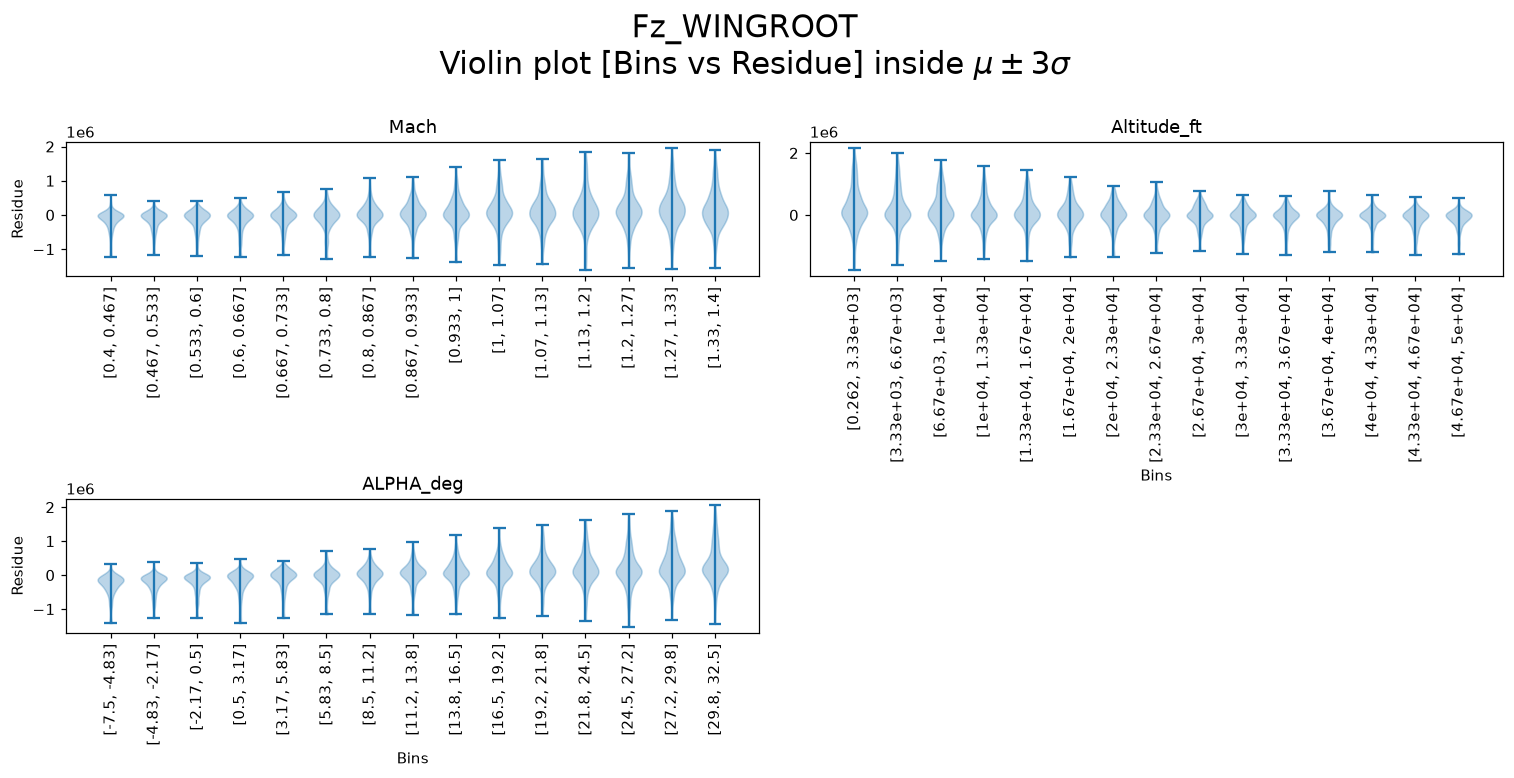
\includegraphics[width=1.0\linewidth,height=0.80\textheight,keepaspectratio]{analysis_plots/pex_violin_res_Fz_WINGROOT.png}\end{center}
\subsection*{\normalsize Residue --- Mx\_WINGROOT}
\begin{center}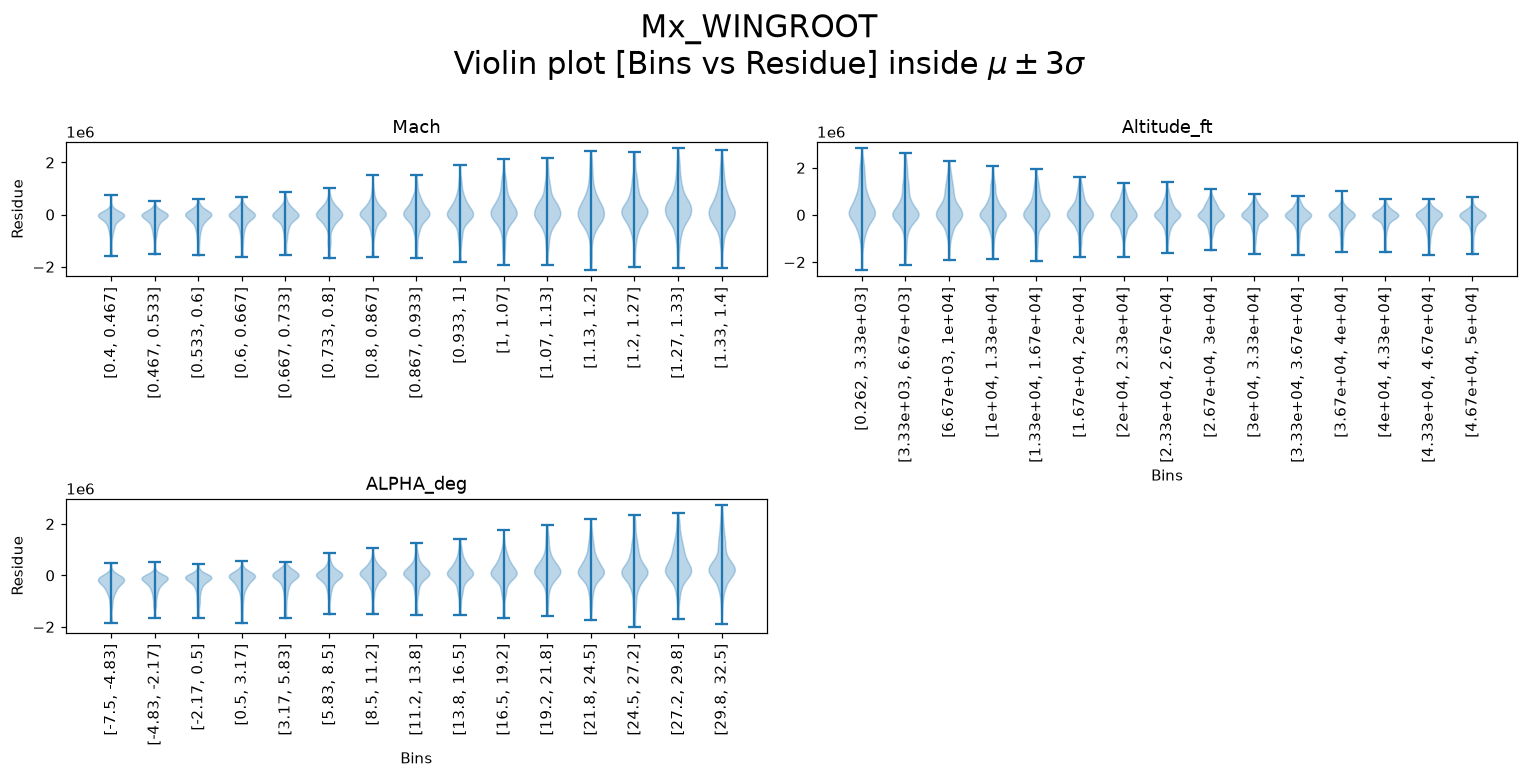
\includegraphics[width=1.0\linewidth,height=0.80\textheight,keepaspectratio]{analysis_plots/pex_violin_res_Mx_WINGROOT.png}\end{center}
\subsection*{\normalsize Residue --- My\_WINGROOT}
\begin{center}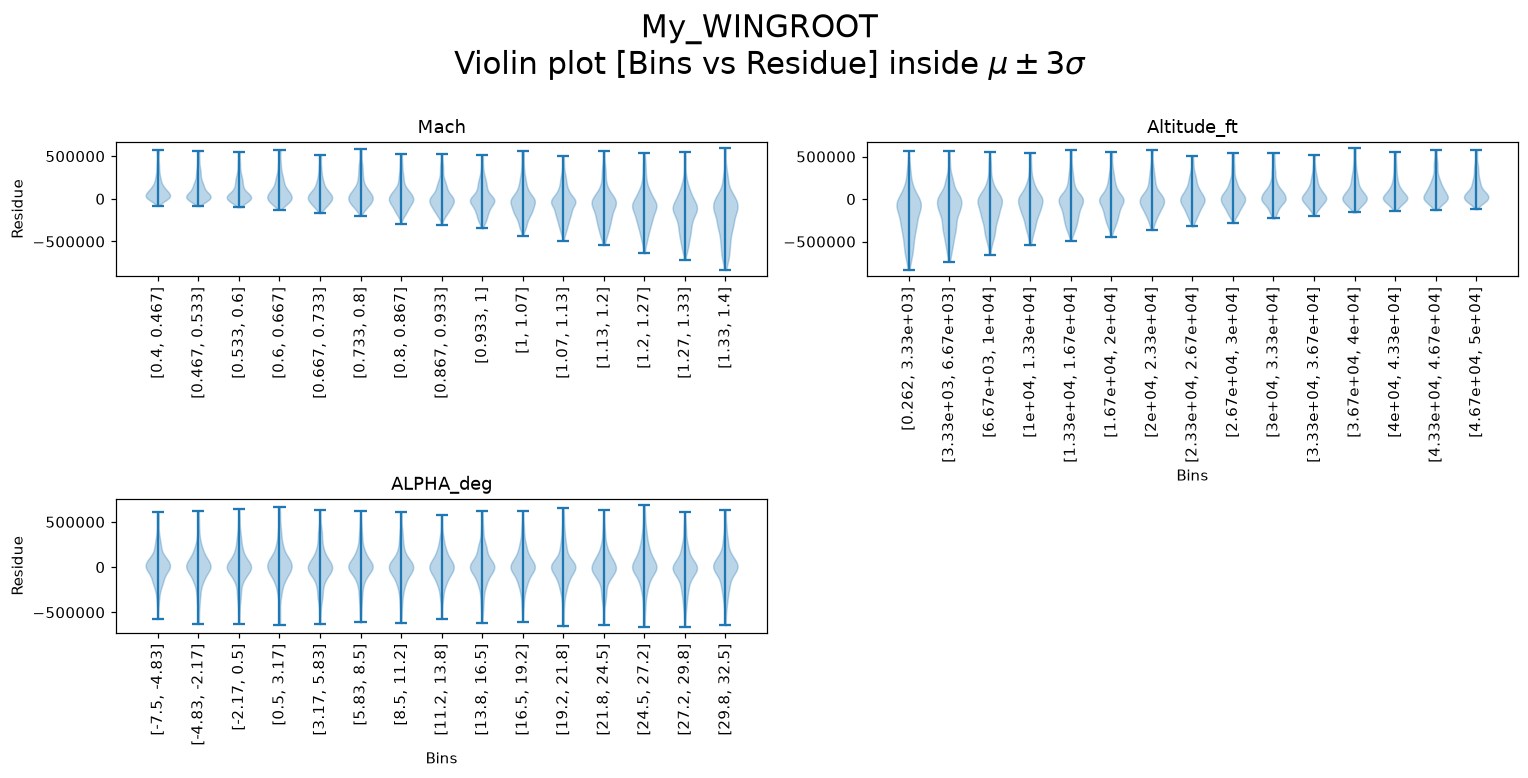
\includegraphics[width=1.0\linewidth,height=0.80\textheight,keepaspectratio]{analysis_plots/pex_violin_res_My_WINGROOT.png}\end{center}
\subsection*{\normalsize Residue --- Fy\_FUS}
\begin{center}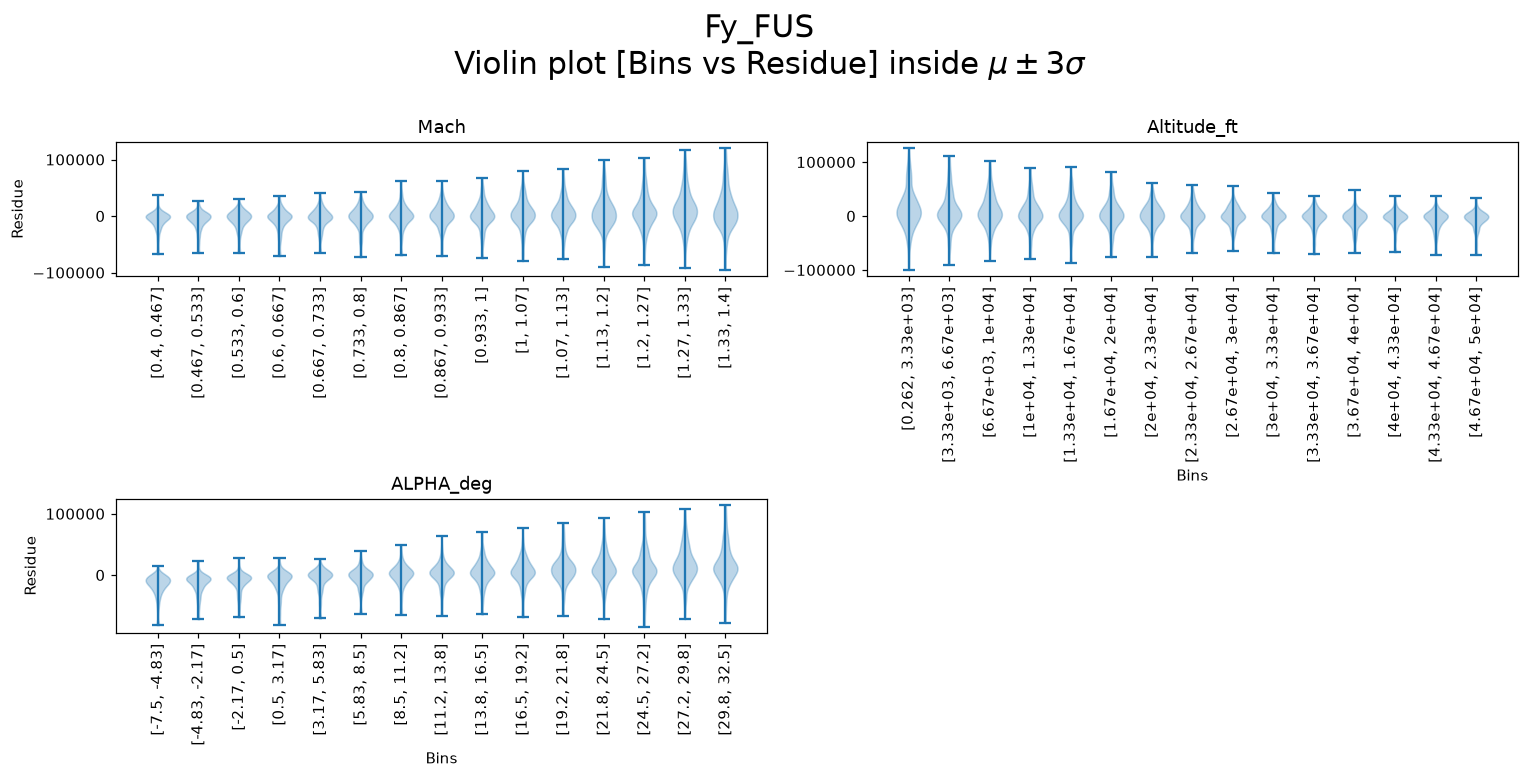
\includegraphics[width=1.0\linewidth,height=0.80\textheight,keepaspectratio]{analysis_plots/pex_violin_res_Fy_FUS.png}\end{center}
\subsection*{\normalsize Residue --- Fz\_FUS}
\begin{center}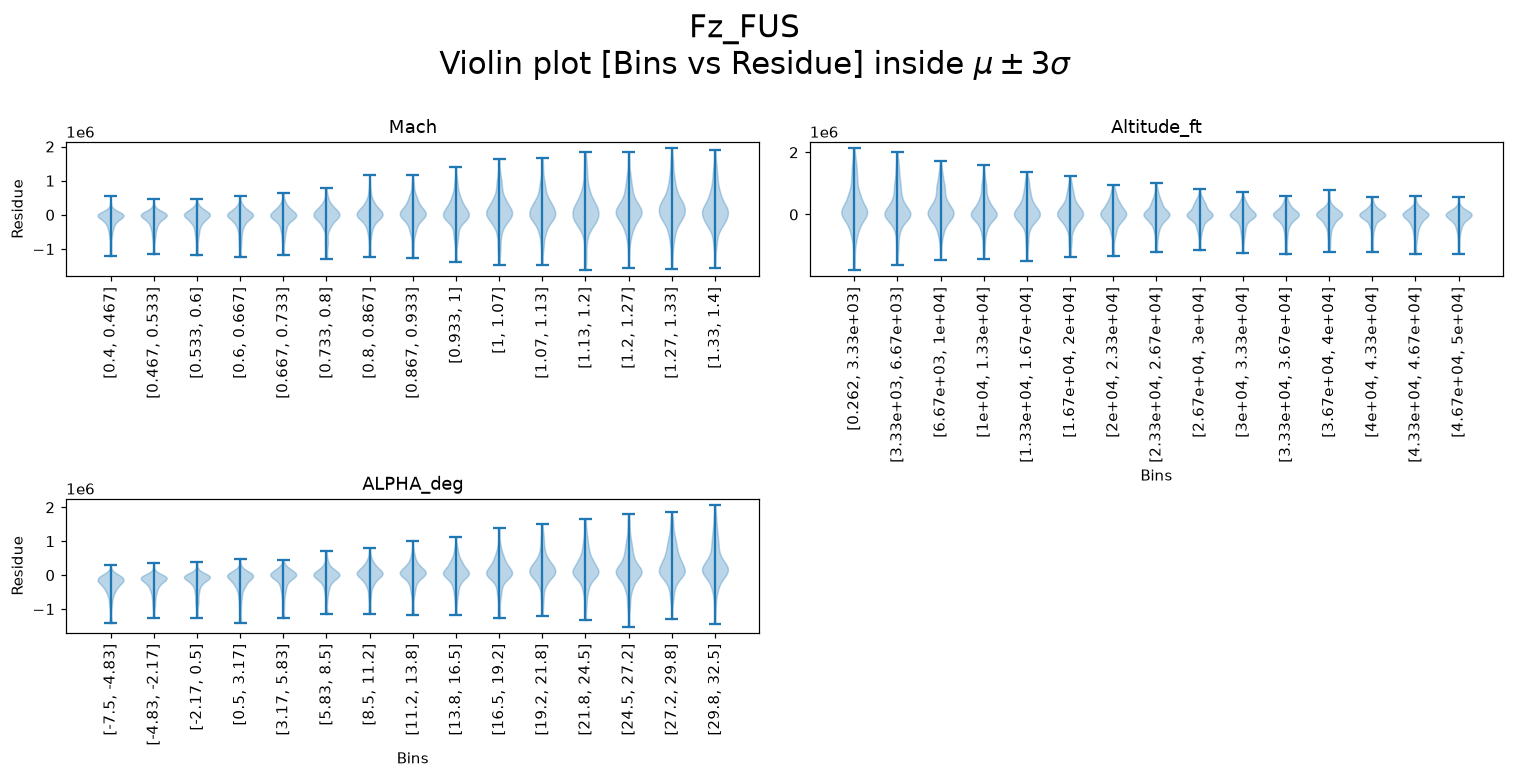
\includegraphics[width=1.0\linewidth,height=0.80\textheight,keepaspectratio]{analysis_plots/pex_violin_res_Fz_FUS.png}\end{center}
\subsection*{\normalsize Residue --- Mx\_FUS}
\begin{center}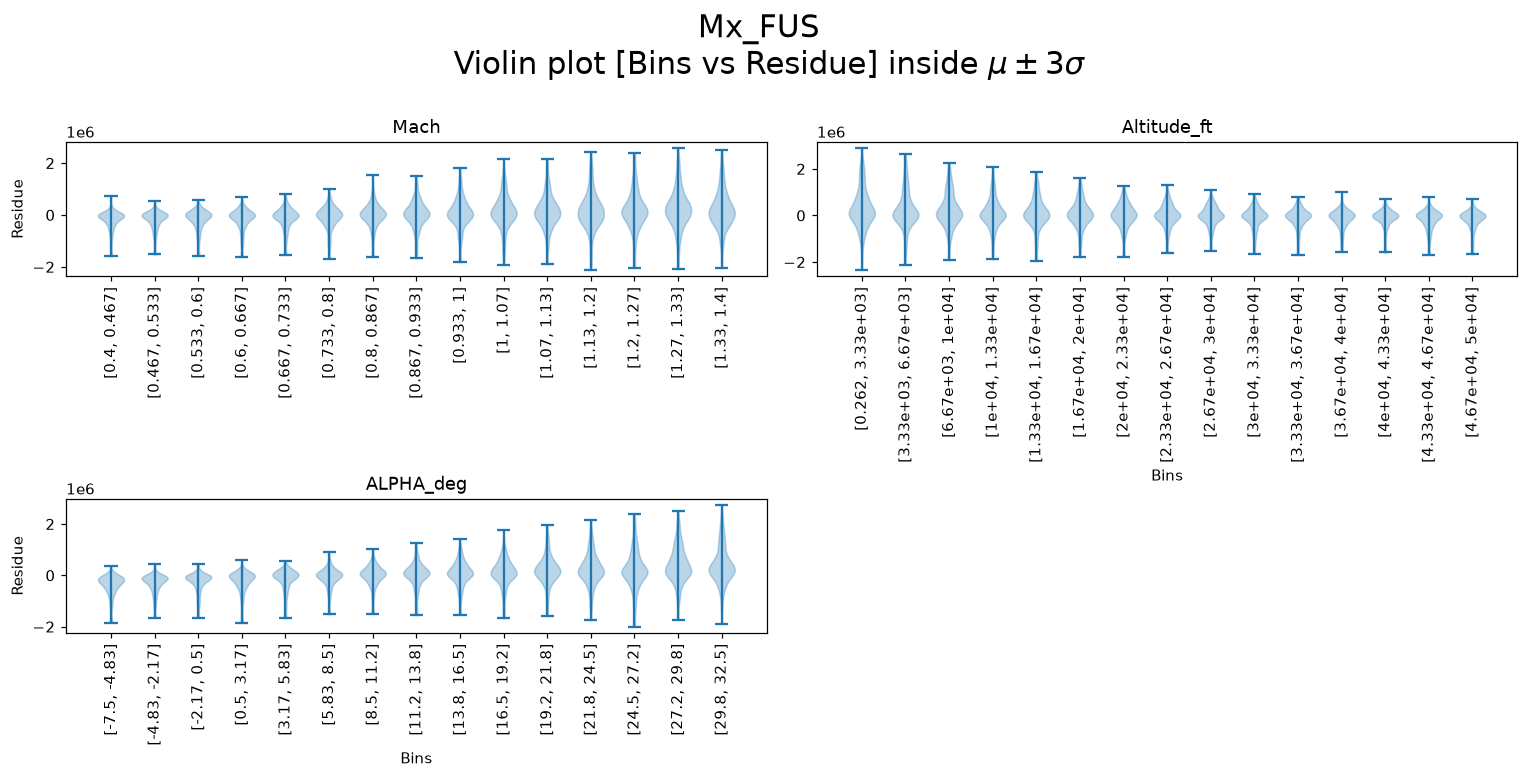
\includegraphics[width=1.0\linewidth,height=0.80\textheight,keepaspectratio]{analysis_plots/pex_violin_res_Mx_FUS.png}\end{center}
\subsection*{\normalsize Residue --- My\_FUS}
\begin{center}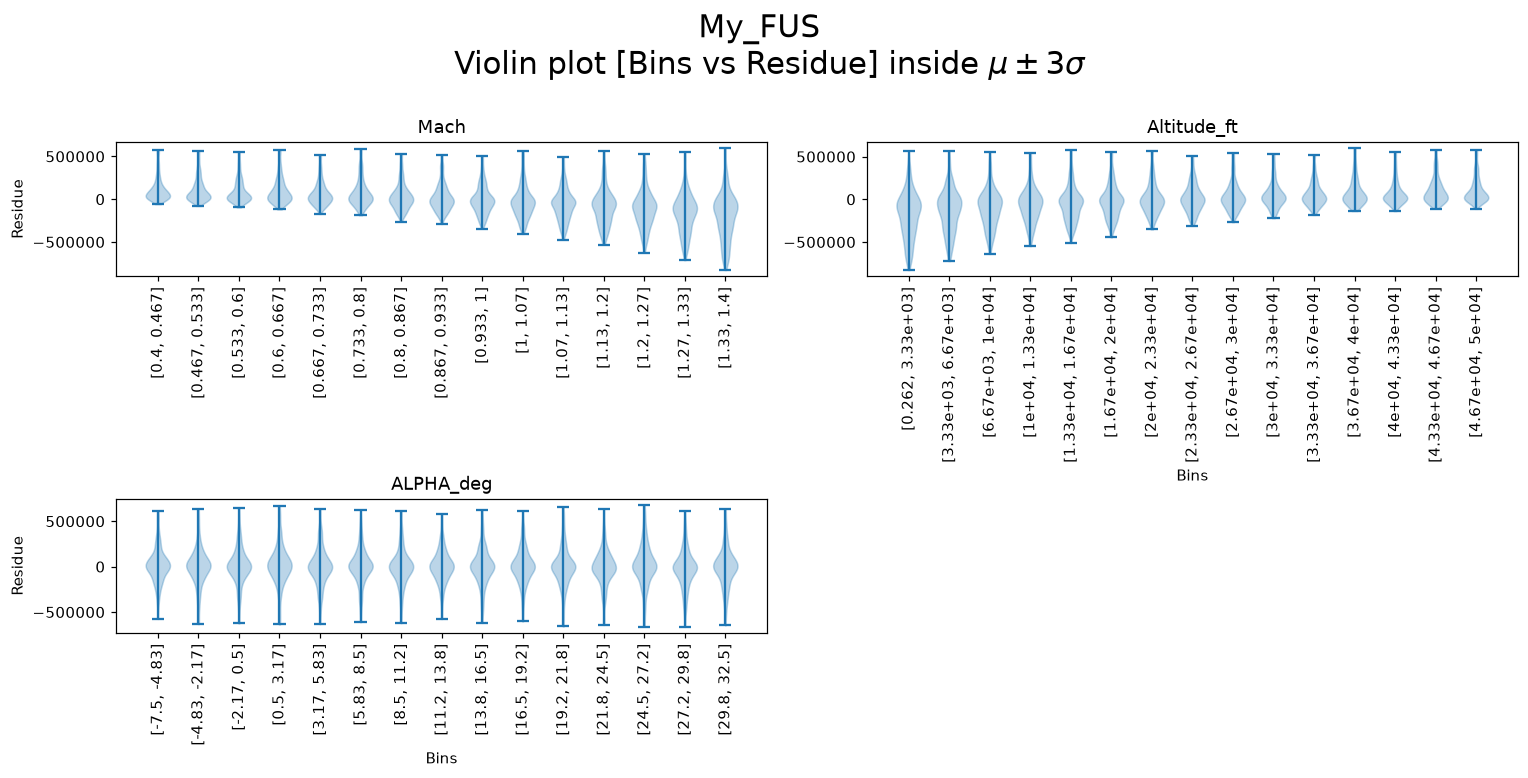
\includegraphics[width=1.0\linewidth,height=0.80\textheight,keepaspectratio]{analysis_plots/pex_violin_res_My_FUS.png}\end{center}
\subsection*{\normalsize Residue --- Mz\_FUS}
\begin{center}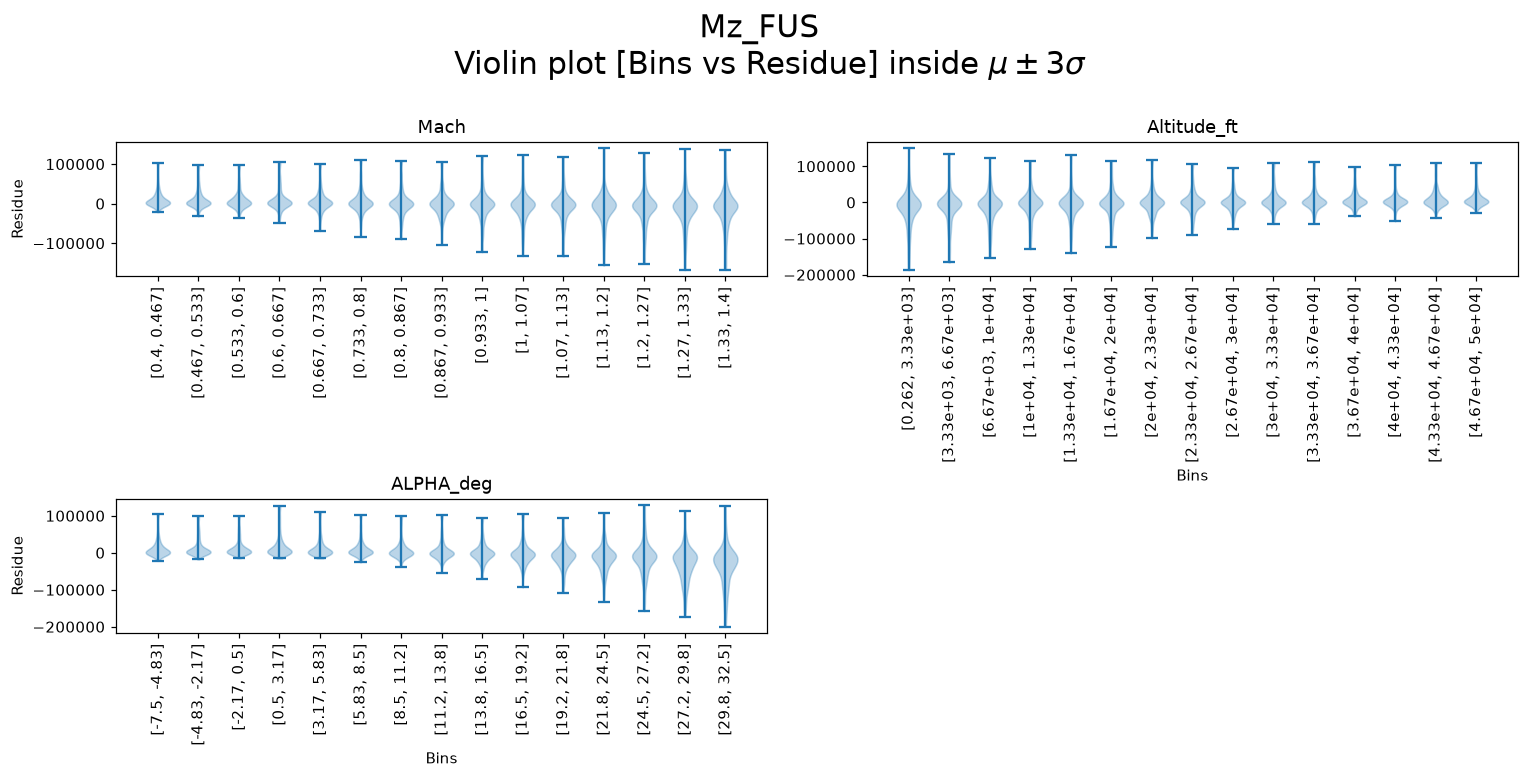
\includegraphics[width=1.0\linewidth,height=0.80\textheight,keepaspectratio]{analysis_plots/pex_violin_res_Mz_FUS.png}\end{center}
\clearpage
\exhead{Absolute Error Violin Plots per Output (binned by input)}
\subsection*{\normalsize Absolute Error --- Fz\_WINGROOT}
\begin{center}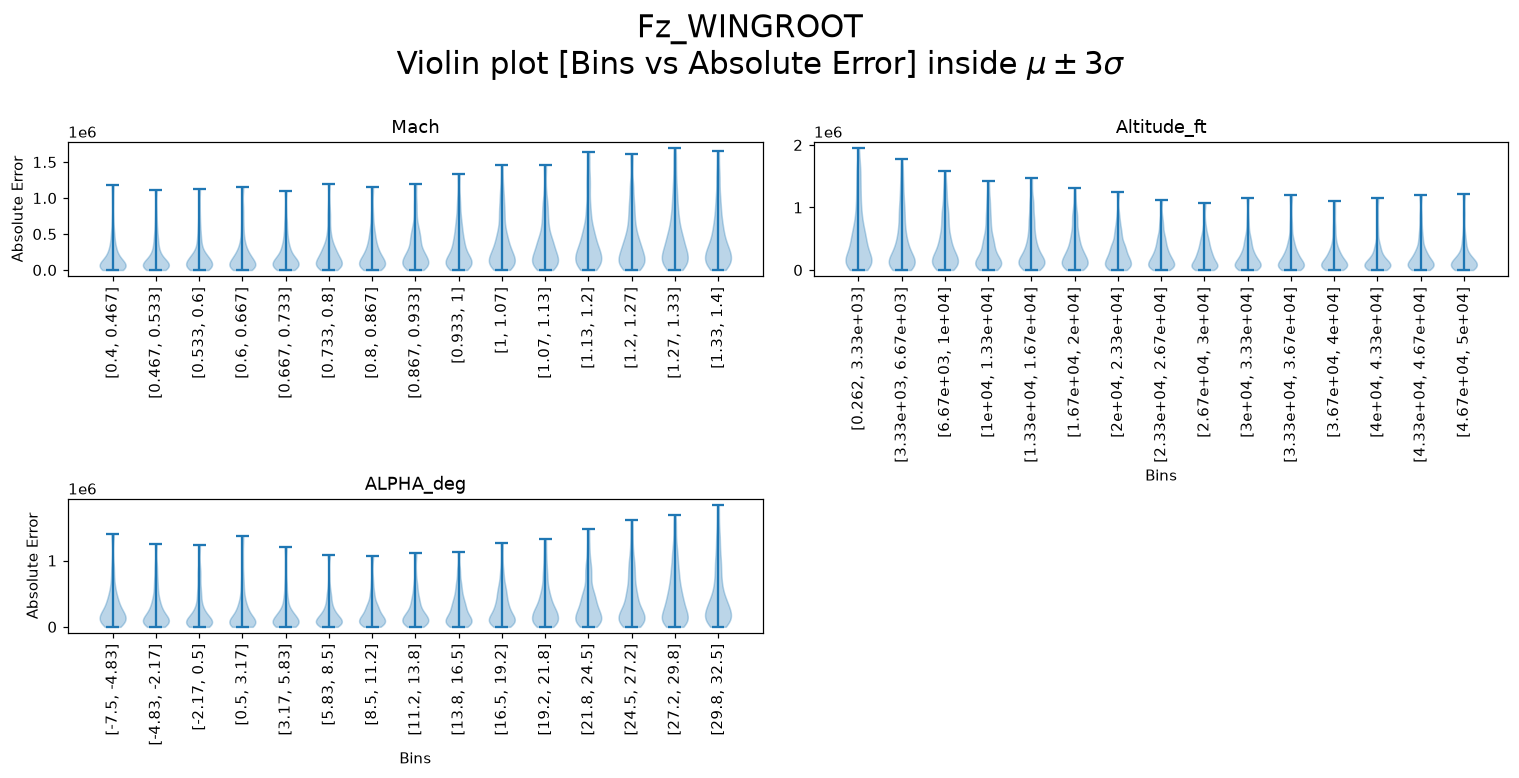
\includegraphics[width=1.0\linewidth,height=0.80\textheight,keepaspectratio]{analysis_plots/pex_violin_abs_Fz_WINGROOT.png}\end{center}
\subsection*{\normalsize Absolute Error --- Mx\_WINGROOT}
\begin{center}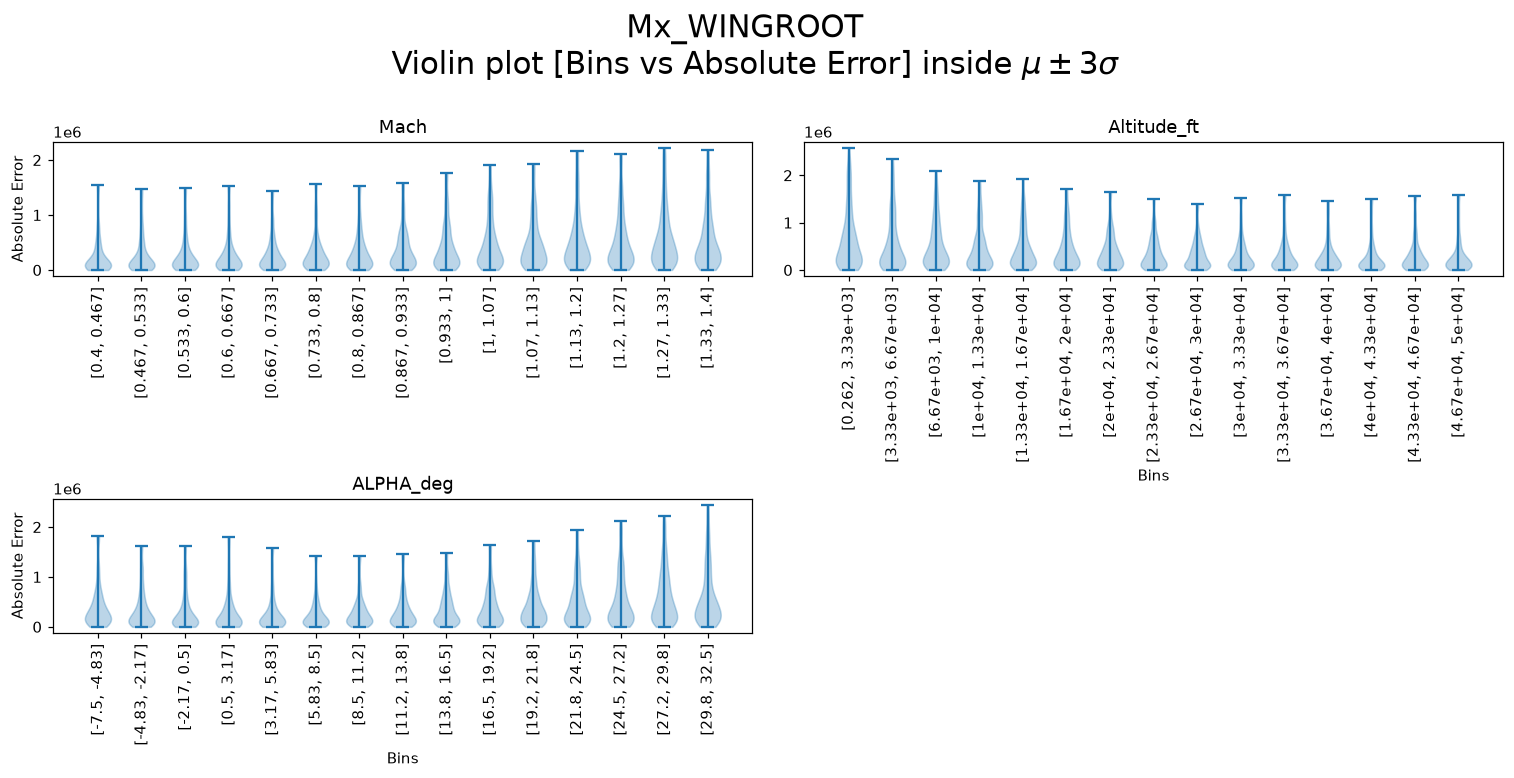
\includegraphics[width=1.0\linewidth,height=0.80\textheight,keepaspectratio]{analysis_plots/pex_violin_abs_Mx_WINGROOT.png}\end{center}
\subsection*{\normalsize Absolute Error --- My\_WINGROOT}
\begin{center}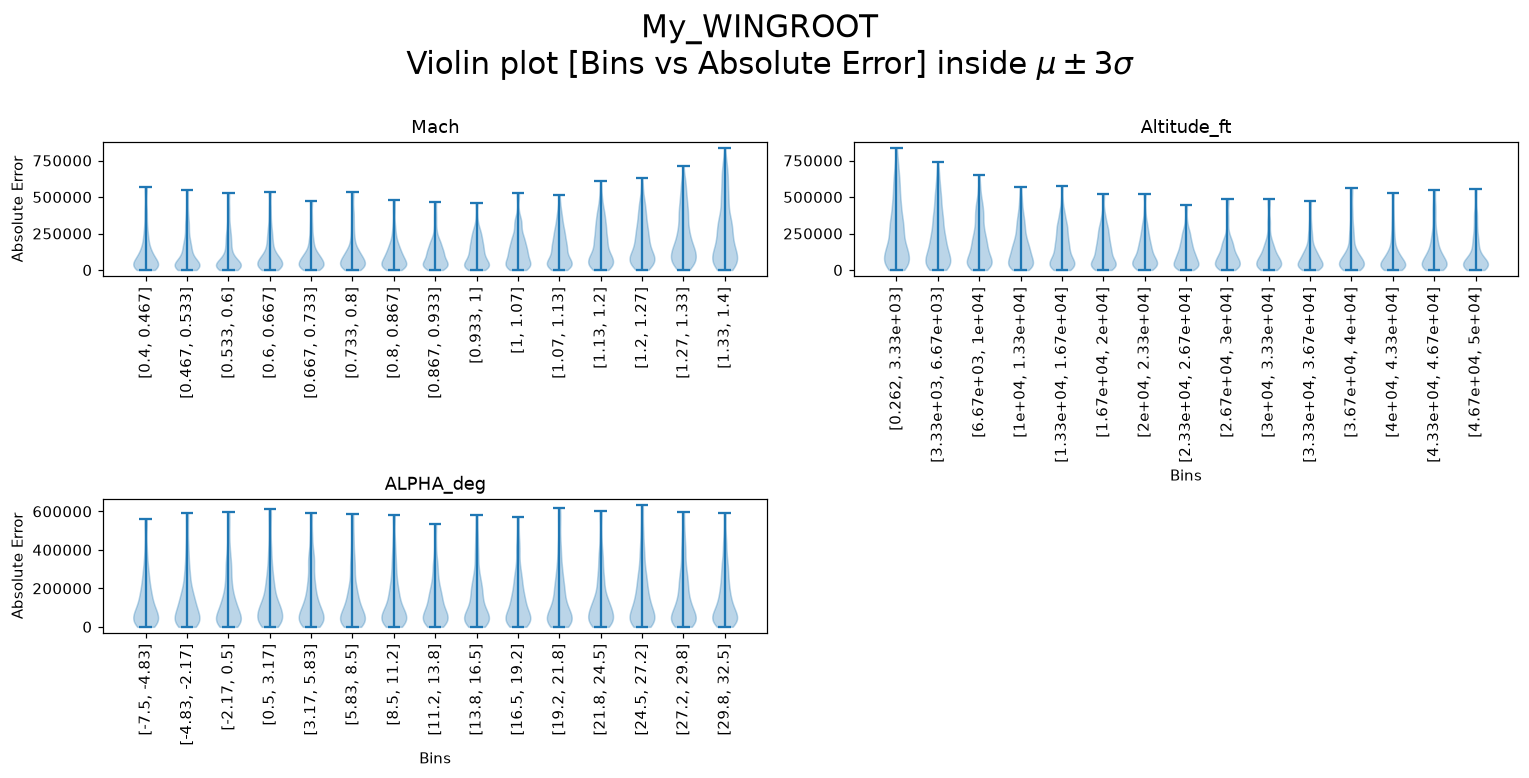
\includegraphics[width=1.0\linewidth,height=0.80\textheight,keepaspectratio]{analysis_plots/pex_violin_abs_My_WINGROOT.png}\end{center}
\subsection*{\normalsize Absolute Error --- Fy\_FUS}
\begin{center}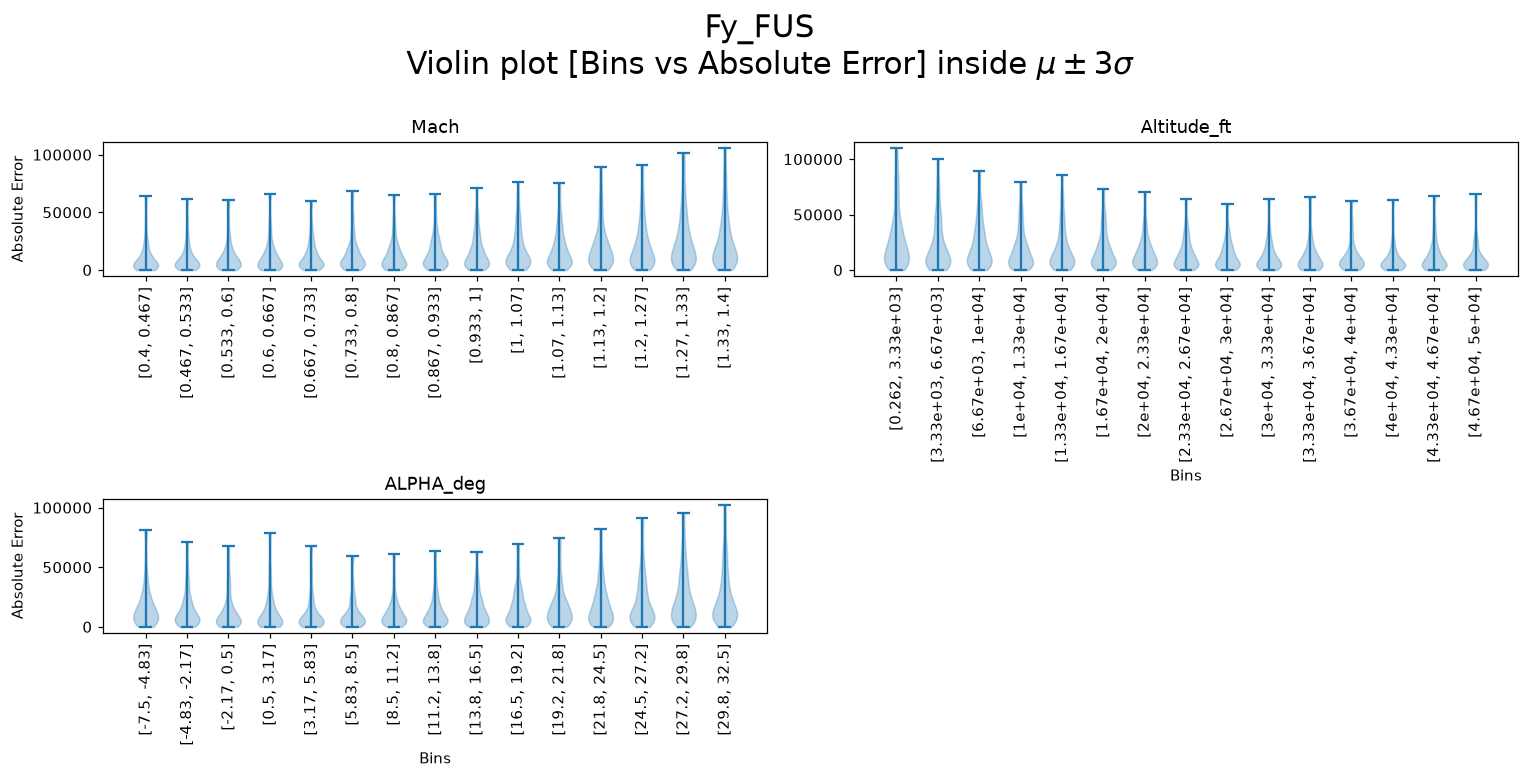
\includegraphics[width=1.0\linewidth,height=0.80\textheight,keepaspectratio]{analysis_plots/pex_violin_abs_Fy_FUS.png}\end{center}
\subsection*{\normalsize Absolute Error --- Fz\_FUS}
\begin{center}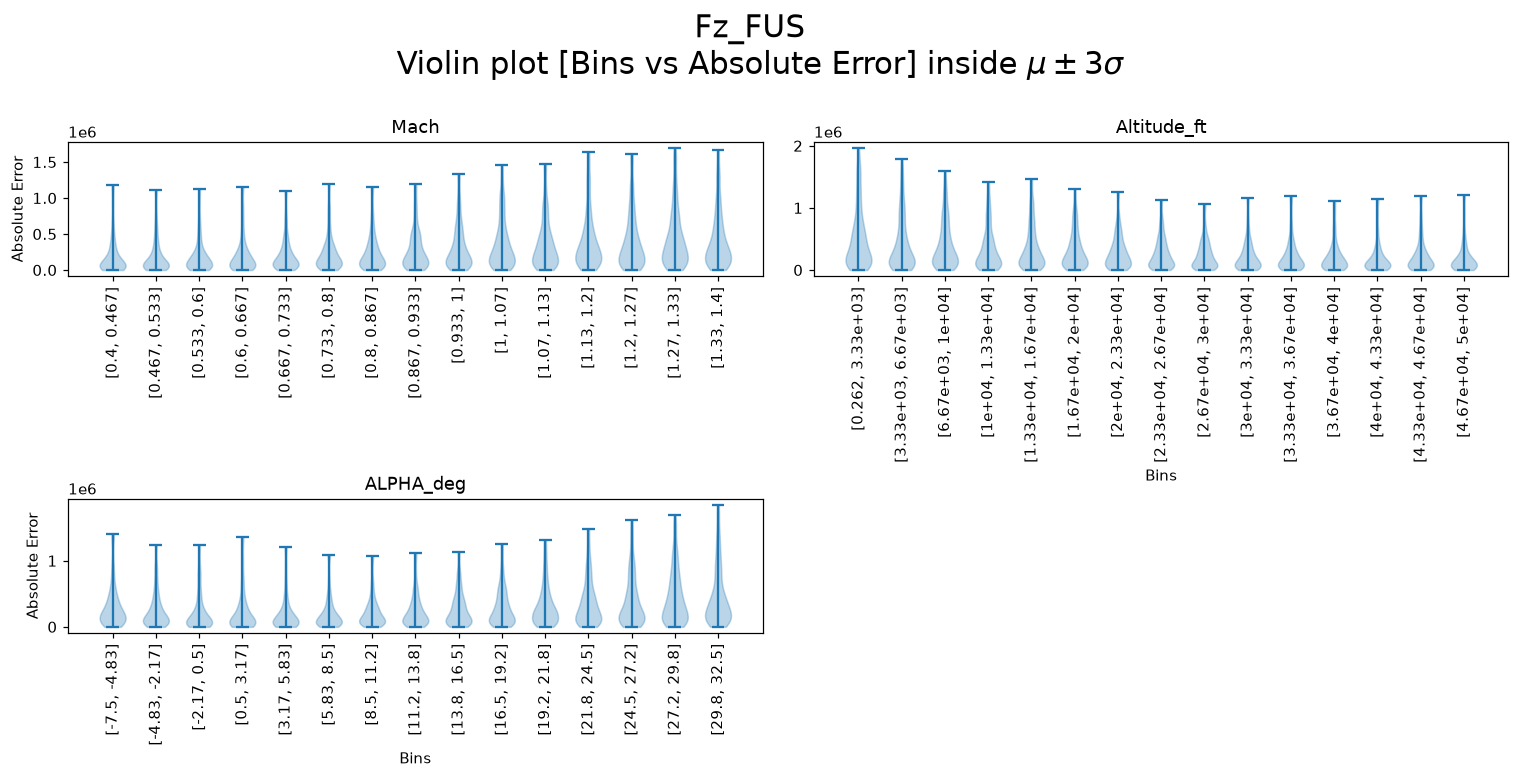
\includegraphics[width=1.0\linewidth,height=0.80\textheight,keepaspectratio]{analysis_plots/pex_violin_abs_Fz_FUS.png}\end{center}
\subsection*{\normalsize Absolute Error --- Mx\_FUS}
\begin{center}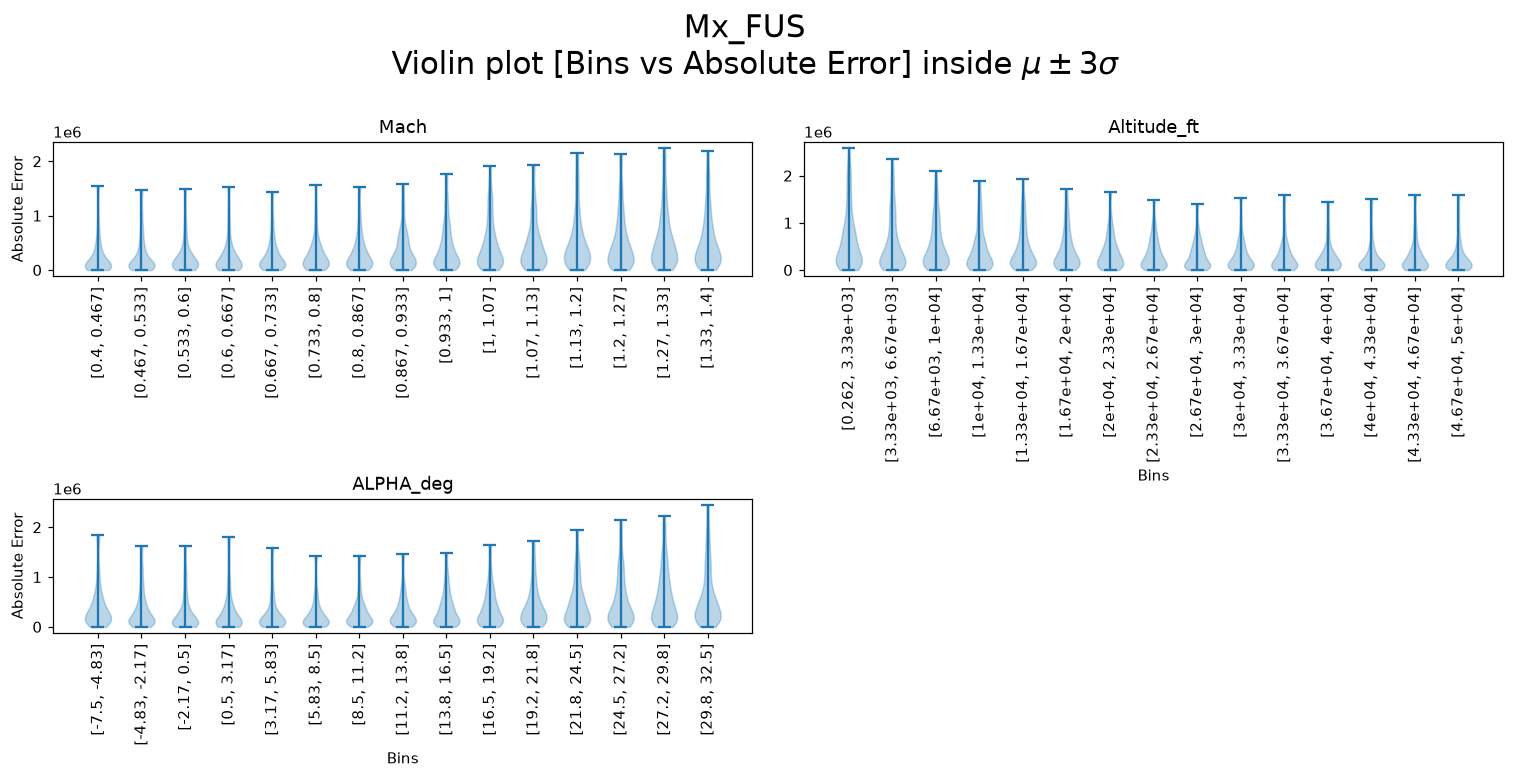
\includegraphics[width=1.0\linewidth,height=0.80\textheight,keepaspectratio]{analysis_plots/pex_violin_abs_Mx_FUS.png}\end{center}
\subsection*{\normalsize Absolute Error --- My\_FUS}
\begin{center}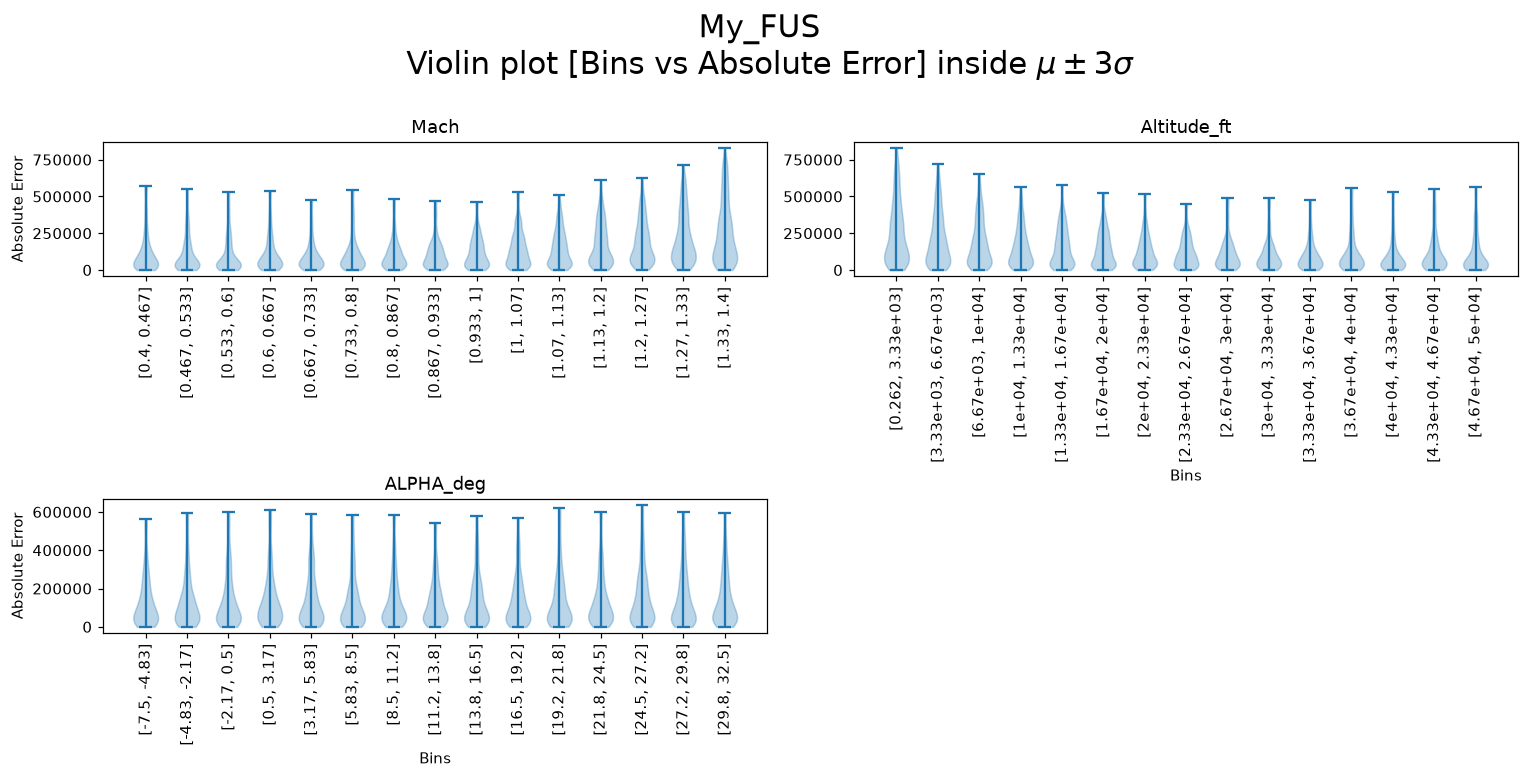
\includegraphics[width=1.0\linewidth,height=0.80\textheight,keepaspectratio]{analysis_plots/pex_violin_abs_My_FUS.png}\end{center}
\subsection*{\normalsize Absolute Error --- Mz\_FUS}
\begin{center}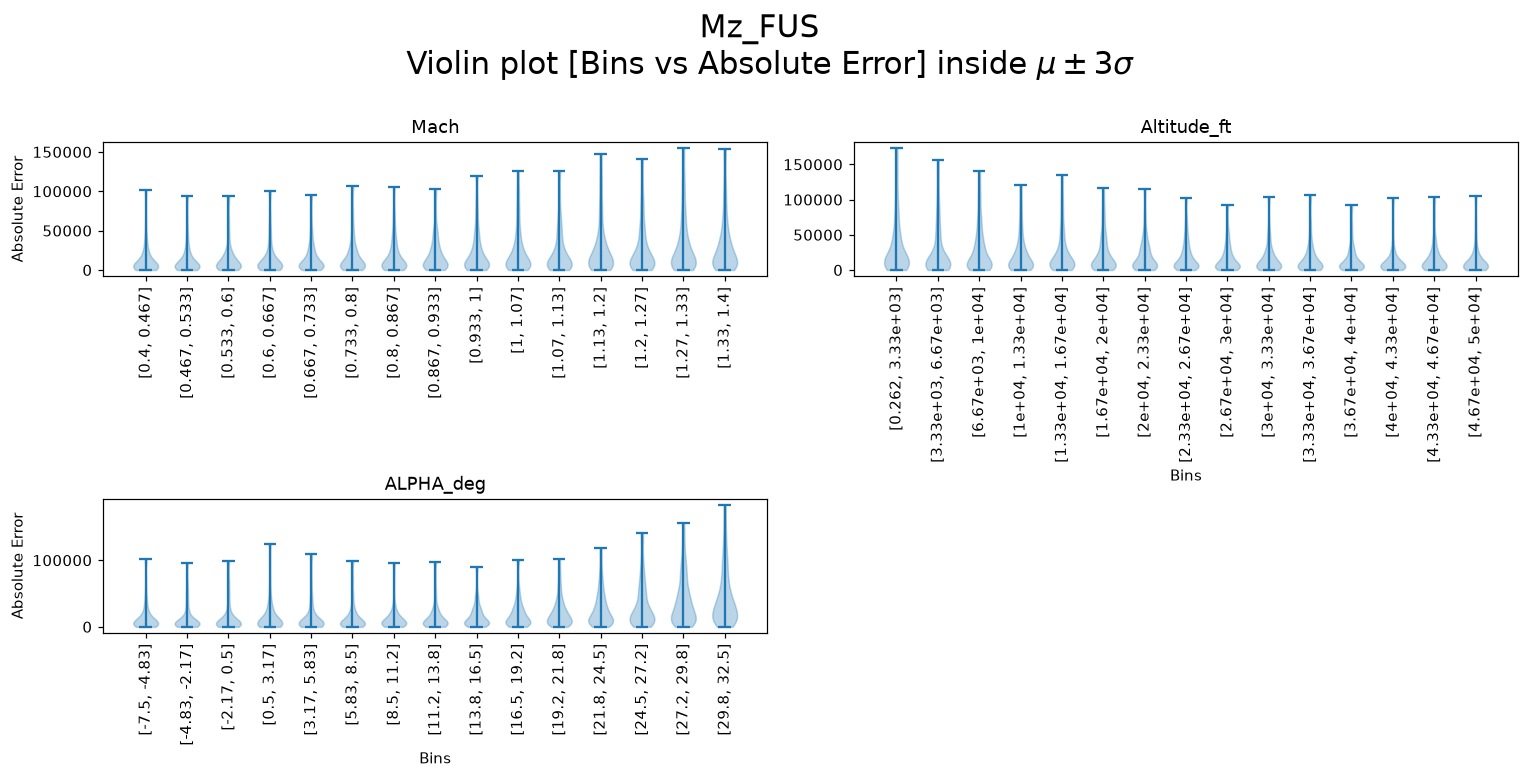
\includegraphics[width=1.0\linewidth,height=0.80\textheight,keepaspectratio]{analysis_plots/pex_violin_abs_Mz_FUS.png}\end{center}
\clearpage
\section{P(E|Y) --- Error Conditional on Outputs}
\label{sec:d5}

We study whether the error depends on the output magnitude. A significant trend (Pearson or Spearman $p<0.05$) means the model is more accurate in some output ranges than others --- a form of heteroscedasticity.

\exhead{Residue vs True Output --- Scatter}
Pearson r and p-value shown in title. Red title = significant linear trend.
\begin{center}
\includegraphics[width=1.0\linewidth,height=0.80\textheight,keepaspectratio]{analysis_plots/pey_residue_scatter.png}\end{center}
\exhead{Residue Violin vs True Output Bins}
Bins determined by Sturges rule. Median line dashed at 0.
\begin{center}
\includegraphics[width=1.0\linewidth,height=0.80\textheight,keepaspectratio]{analysis_plots/pey_residue_violin.png}\end{center}
\exhead{Absolute Error vs True Output --- Scatter}
Spearman r shown. Red title = significant monotonic trend.
\begin{center}
\includegraphics[width=1.0\linewidth,height=0.80\textheight,keepaspectratio]{analysis_plots/pey_abserr_scatter.png}\end{center}
\exhead{Absolute Error Violin vs True Output Bins}
\begin{center}
\includegraphics[width=1.0\linewidth,height=0.80\textheight,keepaspectratio]{analysis_plots/pey_abserr_violin.png}\end{center}
\clearpage
\section{Uncertainty Analysis}
\label{sec:d6}

A global binned uncertainty model (95th percentile, right-tailed) is trained on the validation split of the absolute error and evaluated on the held-out test split, as in the extended validation notebook. Coverage is the proportion of test points whose error falls inside the predicted bound; it should be close to 95\%.

\exhead{Coverage Plot}
\begin{center}
\includegraphics[width=1.0\linewidth,height=0.80\textheight,keepaspectratio]{analysis_plots/uncertainty_coverage.png}\end{center}
\exhead{Coverage Table}
\begin{center}
\footnotesize
\renewcommand{\arraystretch}{1.15}
\resizebox{\linewidth}{!}{%
\begin{tabular}{|l|r|r|r|r|r|r|r|r|r|}
\hline
\textbf{} & \textbf{Fz\_WINGROOT} & \textbf{Mx\_WINGROOT} & \textbf{My\_WINGROOT} & \textbf{Fy\_FUS} & \textbf{Fz\_FUS} & \textbf{Mx\_FUS} & \textbf{My\_FUS} & \textbf{Mz\_FUS} & \textbf{TOTAL COV} \\ \hline
\textbf{Coverage} & 94.55 & 94.54 & 94.77 & 94.39 & 94.72 & 94.54 & 94.77 & 94.07 & nan \\ \hline
\textbf{CI} & [94.09, 94.99] & [94.08, 94.98] & [94.32, 95.2] & [93.92, 94.83] & [94.26, 95.15] & [94.08, 94.98] & [94.32, 95.2] & [93.59, 94.53] & nan \\ \hline
\end{tabular}
}
\par\vspace{2pt}
{\scriptsize Empirical coverage of the 95th-percentile uncertainty bound on the test split.}
\end{center}

\end{document}
